\documentclass[
12pt,				% tamanho da fonte
%openright,		% capítulos começam em pág ímpar (insere página vazia caso preciso)
oneside,			% para impressão no anverso. Oposto a twoside
a4paper,			% tamanho do papel. 
chapter=TITLE,		% títulos de capítulos convertidos em letras maiúsculas
section=TITLE,		% títulos de seções convertidos em letras maiúsculas
%subsection=TITLE,	% títulos de subseções convertidos em letras maiúsculas
%subsubsection=TITLE,% títulos de subsubseções convertidos em letras maiúsculas
% -- opções do pacote babel --
english,			% idioma adicional para hifenização
brazil				% o último idioma é o principal do documento
hyperref=hidelinks]{abntex2}

\usepackage[semdicas]{tccctj} % carrega o estilo CTJ
\bibliographystyle{abntex2-alf-ufsc} % Arquivo bst com patch para correção de citação de proceedings. Produz italico em "In", conforme descrito em: https://github.com/abntex/abntex2/issues/226

% Useful packages
\usepackage{amsmath}
\usepackage{graphicx}
% Pacotes adicionais
\usepackage{multicol}
\usepackage{multirow}
\usepackage{tabularx}
\usepackage{quoting}
\quotingsetup{indentfirst={false},font={footnotesize},leftmargin=4cm,rightmargin=0cm} 
\hypersetup{hidelinks}
\usepackage{enumitem}
\setlist{noitemsep}
%\usepackage{hyperref}
%\usepackage{array,epsfig}
%\usepackage{amsfonts}
%\usepackage{amssymb}
%\usepackage{amsxtra}
%\usepackage{amsthm}
%\usepackage{mathrsfs}
%\usepackage{color}
%\usepackage{indentfirst}
\usepackage{float}
\usepackage{booktabs}
\usepackage{array}
\usepackage{longtable}
\usepackage[nobiblatex]{xurl}
\usepackage{textcomp}

% ----------------------------------------------------

% ----------------------------------------------------
% Informações do trabalho
\autor{Yuri Gazzoni Rezende}
\titulo{Projeto de um Computador de Bordo Robusto e Versátil Para Uso em pequenos satélites}
% \subtitulo{Subtítulo} % Preenchimento opcional para quando houver sub-título
\orientador{Msc. Gabriel Mariano Marcelino}
%\coorientador{Nome do coorientador} % Preenchimento opcional para quando houver co-orientador
\curso{Departamento de Engenharia Elétrica e Eletrônica}
% \titulacao{Bacharel em x}
\datadadefesa{15}{novembro}{2024}
\local{Florianópolis}

\begin{document}

% ----------------------------------------------------
% 1. Capa do trabalho
\imprimircapa

% 2. Folha de rosto
\imprimirfolhaderosto

% 3. Folha de aprovação
\begin{folhadeaprovacao}
    \membrodabanca[Orientador]{Msc. Gabriel Mariano Marcelino}{}
    \membrodabanca{Prof. Dr. Eduardo Bezerra}{UFSC}
    \membrodabanca{Membro da banca 2}{UFSC}
    \membrodabanca{Membro da banca 3}{UFSC}
\end{folhadeaprovacao}

% 4. Dedicatória
%\begin{dedicatoria}
%    Este trabalho é dedicado aos meus colegas de classe e aos meus queridos pais.
%\end{dedicatoria}

% 5. Agradecimentos 
%\begin{agradecimentos}
%   Inserir os agradecimentos aos colaboradores à execução do trabalho.
%\end{agradecimentos}

% 6. Epígrafe
%\begin{epigrafe}
%    \aspas
%    A natureza é um enorme jogo de xadrez disputado por deuses, e que temos o privilégio de observar.
%    As regras do jogo são o que chamamos de física fundamental, e compreender essas regras é a nossa meta.
%    \aspas
%    \autor{Richard Phillips Feynman} % autor da epígrafe
%\end{epigrafe}

% 7. Resumo em português
\begin{resumo}
Este trabalho apresenta o projeto e desenvolvimento de uma arquitetura de hardware para um computador de bordo adequado para pequenos satélites, como CubeSats, que operam em órbitas baixas (LEO). O objetivo principal foi desenvolver uma solução que atendesse aos requisitos críticos do ambiente espacial, integrando componentes comerciais (COTS) selecionados conforme diretrizes de herança de voo e normas da ESA e NASA, assegurando confiabilidade e estabilidade. Para garantir versatilidade, a solução foi baseada em um SoC da família Zynq, que integra um microprocessador e uma FPGA, que permite a mudança da funcionalidade de cada pino de entrada e saída. O projeto adota métodos de escolha de componentes e estimativas de potência. Como resultado, obtém-se um esquemático eletrônico baseado em uma arquitetura com interfaces genéricas, apresentando circuitos que possibilitam futuros desenvolvimentos para missões ou estudos específicos em órbita. Conclui-se que o computador de bordo projetado cumpre as exigências de robustez e flexibilidade para missões espaciais em pequenos satélites.

\palavrachave{CubeSats}
\palavrachave{Computador de Bordo}
\palavrachave{Versatilidade}
\end{resumo}

\begin{resumo}[Abstract]
\begin{otherlanguage*}{english}
This project presents the design and development of a hardware architecture for an on-board computer suitable for small satellites, such as CubeSats, operating in low Earth orbit (LEO). The main objective was to develop a solution that meets the critical requirements of the space environment, integrating commercial components (COTS) selected according to flight heritage guidelines and ESA and NASA standards, ensuring reliability and stability. To ensure versatility, the solution was based on a SoC from the Zynq family, which integrates a microprocessor and an FPGA, allowing the functionality of each input and output pin to be changed. The project adopts methods for choosing components and estimating power. The result is a schematic capture based on an architecture with generic interfaces, featuring circuits that enable future developments for specific missions or studies in orbit. It is concluded that the on-board computer designed meets the requirements of robustness and flexibility for space missions on small satellites.
\vspace{\onelineskip}
\noindent 

\textbf{Keywords}: CubeSats. On-board Computer. Versatility.
 \end{otherlanguage*}
\end{resumo}

% 9. Lista de figuras
\imprimirlistafiguras

% 10. Lista de quadros
%\imprimirlistaquadros

% 11. Lista de tabelas
\imprimirlistatabelas

% 12. Lista de abreviaturas e siglas
\begin{siglas}
	\item[ADC] \textit{Analog to Digital Converter}
	\item[ADCS] \textit{Attitude Determination and Control System}
	\item[CAN] \textit{Controller Area Network}
	\item[COTS] \textit{Commercial-off-the-shelf}
	\item[DDR] \textit{Double Data Rate}
	\item[ECSS] \textit{European Cooperation for Space Standardization}
	\item[EMI] \textit{Electromagnetic Interference}
	\item[ESA] \textit{European Space Agency}
	\item[ESR] \textit{Equivalent Series Resistor}
	\item[FPGA] \textit{Field-Programmable Gate Array}
	\item[HP] \textit{High Performance} 
	\item[HR] \textit{High Range}
	\item[I2C] \textit{Inter-Integrated Circuit}
	\item[JTAG] \textit{Joint Test Action Group}
	\item[LEO] \textit{Low Earth Orbit}
	\item[MEO] \textit{Medium Earth Orbit}
	\item[MIO] \textit{Multiplexed In-Out}
	\item[NASA] \textit{National Aeronautics and Space Administration}
	\item[NPSL] \textit{NASA Part Selection List}
	\item[OBDH] \textit{On-board Data Handling} 
	\item[PCB] \textit{Printed Circuit Board}
	\item[PL] \textit{Programmable Logic}
	\item[PS] \textit{Processing System}
	\item[QSPI] \textit{Quad Serial Peripheral Interface}
	\item[RTC] \textit{Real Time Clock}
	\item[RTOS] \textit{Real Time Operational System}
	\item[SDR] \textit{Single Data Rate}
	\item[SEE] \textit{Single Event Effects}
	\item[SoC] \textit{System-on-a-Chip}
	\item[SPI] \textit{Serial Peripheral Interface}
	\item[TID] \textit{Total Ionizing Dose}
	\item[UART] \textit{Universal Asynchronous Receiver-Transmitter}
	\item[WDT] \textit{Watchdog Timer}	
	\item[XADC] \textit{Xilinx Analog to Digital Converter}
\end{siglas}

% 13. Lista de símbolos 

% 14. Sumário
\imprimirsumario

% ----------------------------------------------------

% Elementos textuais
\textual


\chapter{Introdução}
\label{Chap:intro}

CubeSats são pequenos satélites que atendem a estritas formas de cubos padronizados de 10 cm de aresta, além de pesarem menos de 300 kg. Cada um desses cubos padronizados recebe a denominação de 1U, e os tamanhos subsequentes de 1,5U, 2U, 3U, e assim por diante (CUBESAT Design Specification, 2022). Devido a essa padronização e ao uso de componentes comerciais, os CubeSats podem ser produzidos em massa, o que diminui substancialmente os custos de lançamento e desenvolvimento (CubeSat 101, 2017).

O desenvolvimento de satélites de pequeno porte, como CubeSats e nanosatélites, trouxe novas oportunidades e desafios para a indústria espacial, permitindo que uma ampla gama de missões científicas, comerciais e educacionais fosse realizada com custos reduzidos e prazos de desenvolvimento mais curtos (CUBESAT Design Specification, 2022). No entanto, a miniaturização e a operação em ambientes espaciais impõem requisitos à robustez, confiabilidade e versatilidade dos sistemas embarcados, especialmente para os módulos OBDHs (\textit{On-Board Data Handling}). Nesse contexto, a arquitetura de um computador de bordo eficiente e robusto é essencial para o gerenciamento seguro das operações e para garantir a integridade das missões.

Essa segurança e integridade são pontos chave no desenvolvimento de CubeSats no SpaceLab, laboratório da UFSC especializado em desenvolvimento de sistemas espaciais para a comunidade científica e para a indústria. Um dos objetivos primários do SpaceLab é o desenvolvimento de uma plataforma \textit{open-source}, tanto para \textit{software} quanto \textit{hardware}, o que já foi feito nos desenvolvimentos do FloripaSat-1 (MARCELINO et al., 2020) e FloripaSat-2 (MARCELINO et al., 2024). Com esse paradigma, a oportunidade de se ter um computador de bordo mais robusto (com mais memória e capacidade de processamento) e versátil surgiu, como uma consequência direta dos desenvolvimentos das gerações anteriores de \textit{hardware} do laboratório.

O sistema desenvolvido para o presente trabalho foca na implementação de uma arquitetura de processamento e memória capaz de atender às demandas de um satélite de pequeno porte. Esse sistema deve operar de maneira confiável em ambientes suscetíveis à radiação e alta variação de temperatura, em conjunto com a otimização do uso de energia. Além disso, a versatilidade do computador de bordo é essencial para adaptar o sistema a diferentes tipos de missões, desde operações de imagem e telemetria até experimentos científicos em órbita. Para isso, é necessário que o sistema ofereça uma arquitetura versátil, baseada em uma FPGA (\textit{Field-Programmable Gate Array}), com capacidade de expansão e adaptação a novos sensores e módulos de comunicação.

Inicialmente, será feita uma revisão bibliográfica, explorando as características de computadores de bordo comerciais e de trabalhos acadêmicos, além de entender como a radiação em órbita baixa afeta os sistemas eletrônicos. Depois disso, será definida uma arquitetura, respeitando os requisitos impostos, em conjunto com uma estimativa de consumo de potência. Com a arquitetura, será desenvolvido um esquemático, usando o software Altium Designer (versão 24.4.1). Por fim, serão apresentados os resultados obtidos e as considerações finais e conclusões para esse projeto.

\section{Objetivo geral}

O presente trabalho tem como objetivo o projetar e implementação de uma arquitetura de hardware robusta e versátil para um computador de bordo de satélite de pequeno porte, integrando diferentes tipos de memórias e periféricos para assegurar a operação confiável em ambientes espaciais adversos, garantindo a integridade dos dados e a eficiência no gerenciamento dos mesmos.

\section{Objetivos Específicos}

\begin{itemize}
    \item Analisar os requisitos de robustez em condições espaciais, com foco em resistência a radiação, tolerância a falhas e estabilidade térmica, a fim de assegurar o funcionamento contínuo do computador de bordo em órbita.
    \item Especificar uma arquitetura de hardware que permita a adaptação a diferentes tipos de missões, integrando diferentes tipos de componentes comerciais com um SoC (\textit{System-on-a-chip}).
    \item  Documentar as decisões de projeto para consolidar um guia técnico com recomendações de design para sistemas de robustos e versáteis aplicáveis a satélites de pequeno porte, contribuindo para futuras otimizações e adaptações em missões espaciais.
\end{itemize}

% ----------------------------------------------------------
\chapter{Revisão Bibliográfica}
% ----------------------------------------------------------

Para atingir o objetivo de projetar o \textit{hardware} de um computador de bordo, foi preciso buscar na literatura acadêmica o estado da arte que tange o projeto de OBDHs para satélites de pequeno porte, especialmente para CubeSats.
 
No primeiro tópico, será apresentado um breve estudo sobre a radiação em LEO (\textit{Low Earth Orbit}, órbitas com raio menor que 1000 km, segundo ESA, 2024), para entender os possíveis efeitos em componentes eletrônicos do CubeSat, baseando-se em diferentes autores. Dessa forma, buscaram-se formas de mitigar os efeitos mais conhecidos e verificar como os projetos têm lidado com componentes do tipo \textit{Commercial-Off-The-Shelf} (COTS).% Além disso, também foi dada a fundamentação dos conversores de potência, tipos de memória, microprocessadores e interfaces de comunicação.

Depois disso, serão analisadas diversas placas de computadores de bordo desenvolvidos pela indústria e pela academia, a fim de compreender o estado da arte. Aqui, destacam-se as placas de OBDH dos projetos do FloripaSat-1 e FloripaSat-2, desenvolvidos pelo SpaceLab da UFSC, precursores principais do OBDH a ser desenvolvido nesse trabalho, bem como o Nanomind Z7000, projetado e fabricado pela GomSpace, utilizando um SoC como processador. Um panorama geral será feito, verificando-se principalmente os componentes principais e mais críticos, ou seja, processadores, memórias e outros periféricos.

Por fim, será explicitada a metodologia escolhida para a seleção dos componentes do OBDH projetado, de acordo com o estado da arte e com diretrizes e normas relevantes. Essa explicitação será crucial para que os componentes COTS sejam os melhores possíveis nos quesitos de temperatura e tolerância a falhas.

\section{Radiação em LEO e Componentes COTS}

Estando em solo terrestre, os componentes eletrônicos estão bem protegidos contra a maior parte da radiação incidente do universo, sejam elas raios cósmicos, partículas solares ou \textit{trapped radiation}. No caso dos satélites orbitais, a proteção atmosférica é nula, mesmo para aqueles que operam em LEO. Nesse caso, a radiação pode ser suficientemente significativa para causar a mudança do comportamento eletromagnético dos materiais, causando efeitos como falhas, aquisição ou execução errada de comandos e distorções dos sinais (MAYANBARI, 2011) (LABEL, 2004).  Esses danos são divididos em dois grupos (JUNQUEIRA, 2020): os acumulativos como o TID (\textit{Total Ionizing Dose}), e os SEE (\textit{Single Event Effects}), que indicam o acontecimento de eventos únicos. 

O TID (Figura \ref{fig:tid}), segundo Junqueira (2020), se caracteriza principalmente pela formação de pares elétron-lacuna, onde o primeiro aumenta a condutividade do material e o segundo contribui para oxidação, mudando as características elétricas do componente com o tempo.  Já os SEE (Figura \ref{fig:see}) ocorrem quando um íon atravessa um componente crítico, gerando uma linha de ionização que pode ou não ser destrutiva. 

\begin{figure}[H]
    \centering
    \caption{Esquema representativo do TID.}
    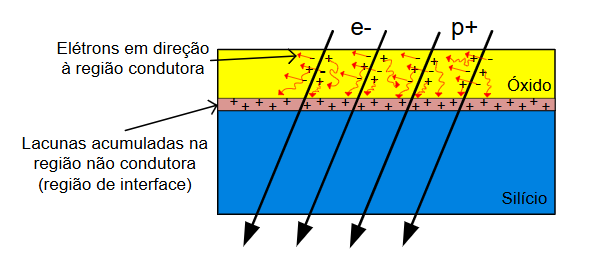
\includegraphics[scale=0.8]{images/tid.png}
    \label{fig:tid}
    \fonte{JUNQUEIRA, 2020.}
\end{figure}

\begin{figure}[H]
    \centering
    \caption{Esquema representativo do SEE.}
    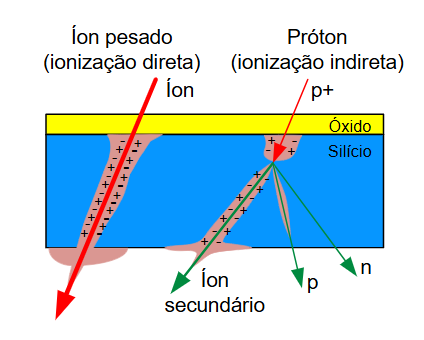
\includegraphics[scale=0.8]{images/see.png}
    \label{fig:see}
    \fonte{JUNQUEIRA, 2020.}
\end{figure}

Especialmente nesse trabalho, o efeito denominado SEL (\textit{Single Event Latch-up}) tem seu destaque. Por ser um tipo de SEE, ocorre após uma partícula carregada atravessar e atingir o substrato do circuito integrado, gerando correntes parasitas que podem ser superiores ao valor máximo suportado pelo componente (JUNQUEIRA, 2020). Proteger os barramentos de alimentação contra esse efeito será crucial para a arquitetura proposta nesse trabalho.

Por esse motivo, quando são escolhidos os componentes críticos para o \textit{hardware} de um \textit{CubeSat}, em sua maioria COTS, deve-se levar em consideração algumas diretrizes principais. Segundo Carmo et al. (2021), o componente escolhido precisa atender os requisitos operacionais, concomitante ao gerenciamento de riscos com mitigações (uso de FRAM, proteção contra \textit{latch-up}, entre outros) e blindagens (uso de \textit{shields} de metal). 

Outro aspecto da seleção de componentes será explorado na seção a seguir, avaliando os OBDHs comerciais e da academia, explorando a característica de herança de voo.

\section{Projetos Anteriores}

\subsection{FloripaSat-1}
% https://ieeexplore.ieee.org/abstract/document/9085277
O FloripaSat-1 (MARCELINO et al., 2020) é uma plataforma \textit{open-source} para nanossatélites, além de ser também o nome do primeiro satélite inteiramente desenvolvido e lançado pelo SpaceLab. O satélite FloripaSat-1 é um CubeSat 1U,  composto de três módulos: um módulo de fornecimento de potência (EPS), um computador de bordo (OBDH) e um módulo de telemetria e comunicação (TTC). Além disso, possuía duas cargas úteis que consistiam de placas com FPGAs. A missão tinha como objetivos a validação do satélite em órbita dos módulos desenvolvidos na UFSC e de um módulo com um FPGA tolerante a radiação.

Seu OBDH foi feito para realização da interface e comunicação entre os módulos e \textit{payloads}. Aqui, destacam-se os sensores presentes: uma \textit{Inertial Measurement Unit} (com giroscópio, magnetômetro e acelerômetro), a interface com os sensores dos painéis solares e as medições de tensão e corrente de entrada do próprio módulo.

Além disso, contava com um microprocessador de 16 bits (MSP430), memórias flash (IS25LP128) e suporte para cartão microSD para armazenamento.

\subsection{FloripaSat-2}
% https://ieeexplore.ieee.org/abstract/document/10078027
O FloripaSat-2 é a segunda geração da plataforma \textit{open-source} desenvolvida pelo SpaceLab, baseando-se no projeto FloripaSat-1 e trazendo melhorias para os três módulos principais (MARCELINO et al., 2024). O diagrama de blocos do CubeSat proposto está disposto na Figura \ref{fig:floripasat2}, onde pode-se verificar as interfaces do OBDH com o restante do módulo.

\begin{figure}[H]
    \centering
    \caption{Diagrama de blocos da plataforma FloripaSat-2.}
    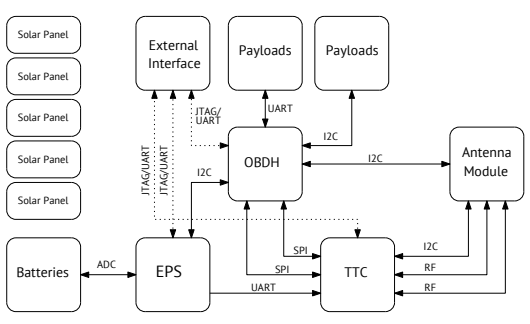
\includegraphics[scale=0.8]{images/floripasat2.png}
    \label{fig:floripasat2}
    \fonte{MARCELINO et al., 2024.}
\end{figure}

Especificamente para o OBDH, foram introduzidas uma memória FRAM (\textit{Ferroelectric Random-Access Memory}) e uma Flash NOR de maior capacidade de armazenamento, o que mostra uma melhoria clara de capacidade e confiabilidade. Outras duas melhorias importantes foram, primeiramente, a adição de um conector para eventualmente conectar uma \textit{daughter board} à placa, e, segundamente, a adição de \textit{buffers} aos barramentos de I2C (\textit{Inter-Integrated Circuit}) entre os módulos. Isso acrescenta flexibilidade e confiabilidade ao OBDH da segunda geração. Esse projeto será utilizado nas missões GOLDS-UFSC, Catarina-A1 e A3 e Aldebaran-1, que ainda não foram lançadas.

\subsection{Projetos Comerciais}

Abaixo se encontram sintetizados os projetos comerciais estudados, para obtenção de noções sobre a arquitetura e componentes usados. Foram verificados principalmente os processadores, as memórias voláteis e não-voláteis, as interfaces de comunicação e outros periféricos (ADCs, RTC, etc.) utilizados. A Tabela \ref{tab:Tab_Rev} mostra a pesquisa realizada sobre o estado da arte, em conjunto com os dados de George e Wilson (2018), sintetizados na Tabela \ref{tab:Tab_Missoes}.

\begin{table}[htb]
    \centering
	\ABNTEXfontereduzida
	\caption{\label{tab:Tab_Rev}Comparação entre os principais modelos comerciais de OBDH disponíveis atualmente no mercado.}
	%\begin{tabular}{@{}p{2cm}p{2cm}p{2cm}p{2cm}p{2cm}p{2cm}p{3cm}@{}}
    \begin{tabular}{@{}p{2cm}p{2.6cm}p{2cm}p{2cm}p{2.2cm}p{2.6cm}@{}}
		\toprule
		\textbf{Fabricante} & \textbf{Nome do Produto} & \textbf{Processador} & \textbf{Memórias} & \textbf{Periféricos} & \textbf{Interfaces de comunicação} \\ 
        \midrule
        GomSpace & NanoMind A3200 & AT32UC3C & Flash, SDRAM, FRAM & Giroscópio, Magnetômetro, Transceivers, Sensores de temperatura & CAN, I2C, SPI, JTAG, USART \\%https://gomspace.com/UserFiles/Subsystems/datasheet/gs-ds-nanomind-a3200_1006901-117.pdf
        
        \midrule
        GomSpace & NanoMind HPMK3 & Zynq 7030 & Flash, eMMC, DDR3 & Watchdog, Sensores de temperatura, VCO, Sensores de tensão e corrente & CAN, USART, USB, I2C, JTAG, LVDS, SpaceWire \\ %https://gomspace.com/UserFiles/Subsystems/datasheet/gs-ds-NanoMind_HP_MK3.pdf

        \midrule
        ISIS Space & ISIS On Board Computer & Atmel & Flash, SDRAM, FRAM, Cartões SD & Sensores de temperatura, Sensores de tensão e corrente, RTC, ADC & USART, USB, I2C, JTAG, PWM \\ %https://www.isispace.nl/product/on-board-computer/

        \midrule
        Nano Avionics & SatBus 3C2 & Não informado & Flash, FRAM, Cartões SD & Giroscópio, Magnetômetro, Rádio UHF, ADC & CAN, SPI, I2C, USART, PWM, USB \\ %https://nanoavionics.com/cubesat-components/cubesat-on-board-computer-main-bus-unit-satbus-3c2/

        \midrule
        AAC Clyde Space & Kryten-M3 & Smart Fusion 2 SoC & MRAM, eNVM & RTC, Sensores de tensão e corrente & CAN, SPI, I2C, USART, RS422, LVDS \\ %https://www.aac-clyde.space/what-we-do/space-products-components/command-data-handling/kryten-m3       


		
        \\ \bottomrule
	\end{tabular}
	\fonte{Elaboração própria.}
\end{table}

\begin{table}[H]
	\ABNTEXfontereduzida
	\caption{\label{tab:Tab_Missoes}Síntese da tabela apresentada por George e Wilson (2018).}
	%\begin{tabular}{@{}p{2cm}p{2cm}p{2cm}p{2cm}p{2cm}p{2cm}p{3cm}@{}}
    \centering
    \begin{tabular}{@{} >{\centering}p{3.5cm} >{\centering}p{3.5cm} >{\centering}p{3.5cm} @{}}
    
		\toprule
		\textbf{Fabricante} & \textbf{Processadores} & \textbf{Missões por Fabricante} \tabularnewline 
        \midrule
        Xilinx & Zynq 7020, Zynq 7030, Zynq 7045, Ultrascale+, etc. & 24 \tabularnewline
        
        \midrule
        Atmel + Microchip & ATmega329P, AT91SAM9G20, PIC24F, etc. & 22 \tabularnewline 

        \midrule
        Texas Instruments & MSP430, OMAP3530, Sitara AM3703, etc. & 15 \tabularnewline 

        \midrule
        Cobham Gaisler & GR712RC, UT699, LEON3FT & 8 \tabularnewline
        
        \bottomrule
	\end{tabular}
	\fonte{Elaboração própria com base em George e Wilson, 2018, página 463.}
\end{table}

Comparando ambas tabelas, é possível verificar que a maioria dos processadores apresentados, no contexto explorado por (GEORGE E WILSON,  2018), são de duas fabricantes: Xilinx (especialmente \textit{chips} da família Zynq 7000) e Microchip (incluindo Atmel). Além disso, a maior parte dos projetos comerciais vistos apresentam memórias FRAM, que possuem um número máximo de ciclos de leitura e escrita muito elevada, além de memórias Flash. Outro destaque foi a presença de sensores de tensão e corrente, bem como magnetômetros e giroscópios.

Além disso, projetos como o OBDH Nanomind Z7000 (GomSpace Nanomind Z7000 Datasheet, 2019) demonstraram sua efetividade em diversas missões, como FSSCAT (CAMPS et al., 2018), ORCA (BARLES et al., 2022) e CubeMAP (WEIDMANN et al., 2020), o que mostra a confiabilidade e herança de voo de \textit{hardwares} contendo SoCs (\textit{System-on-a-Chip}) da família Zynq 7000. Na Figura \ref{fig:nanomind}, podemos verificar o diagrama de blocos do anteriormente citado Nanomind Z7000.

\begin{figure}[H]
    \centering
    \caption{Diagrama de blocos do OBDH Nanomind Z7000.}
    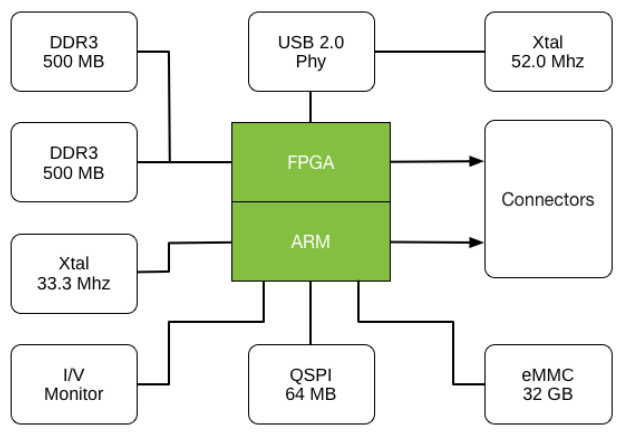
\includegraphics[scale=0.8]{images/nanomind z7000.png}
    \label{fig:nanomind}
    \fonte{GomSpace Nanomind Z7000 Datasheet, 2019.}
\end{figure}

\subsection{Projetos Acadêmicos}

Outro ponto são os OBDHs propostos em publicações acadêmicas. Serão estudados quatro casos de design de OBDH, ainda no contexto de nanossatélites. 

No primeiro caso, o OBDH foi feito para ser compacto e reconfigurável, como o projeto proposto nesse trabalho. O sistema foi pensado para conter um processador, SDRAMs, uma Flash NOR, uma Flash NAND, uma FPGA e algumas interfaces externas (ZHOU et al., 2018). O diagrama de blocos do OBDH proposto pelos autores está disposto na Figura \ref{fig:zhou}.

\begin{figure}[H]
    \centering
    \caption{Diagrama de blocos do OBDH proposto por ZHOU et al., 2018.}
    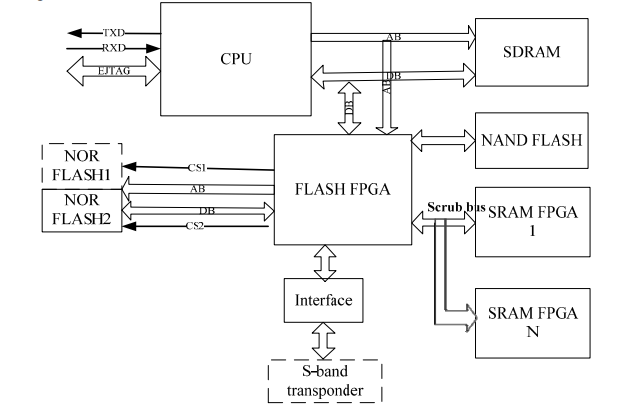
\includegraphics[scale=0.8]{images/zhou.png}
    \label{fig:zhou}
    \fonte{ZHOU et al., 2018.}
\end{figure}

Na segunda publicação estudada, o OBDH é parte de um sistema que implementa um sistema operacional em tempo real (RTOS), outro objetivo desse trabalho. Nesse caso, o OBDH é capaz de verificar telecomandos, sincronizar sistemas, reportar eventos e monitorar parâmetros (PUTRA, 2021). Seu diagrama de blocos do \textit{hardware} está disposto na Figura \ref{fig:putra}.

\begin{figure}[H]
    \centering
    \caption{Diagrama de blocos do OBDH proposto por PUTRA, 2021.}
    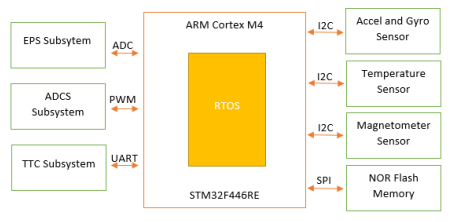
\includegraphics[scale=0.8]{images/putra.png}
    \label{fig:putra}
    \fonte{PUTRA, 2021.}
\end{figure}

No terceiro caso, a missão incluía a pesquisa e observação em órbita média (MEO), ou seja, em condições mais críticas do que o propósito do OBDH projetado nesse trabalho. Mesmo assim, as noções da arquitetura proposta são muito parecidas com o estado da arte para LEO, usando inclusive um SoC da família Zynq 7000 (LOFFLER, 2021). O diagrama de blocos do OBDH proposto nesse trabalho está disposto na Figura \ref{fig:loffler}.

\begin{figure}[H]
    \centering
    \caption{Diagrama de blocos do OBDH proposto por LOFFLER et al., 2021.}
    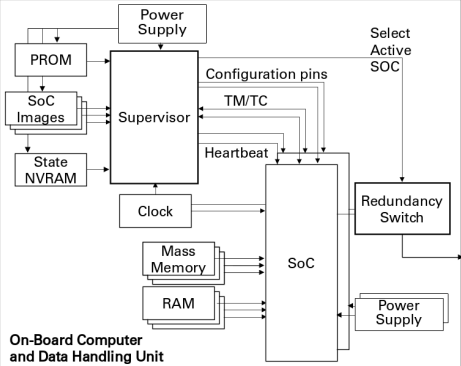
\includegraphics[scale=0.8]{images/loffler.png}
    \label{fig:loffler}
    \fonte{LOFFLER et al., 2021.}
\end{figure}

Nos três casos existem semelhanças na arquitetura, incluindo memórias usadas e interfaces de comunicação. Com isso, juntamente com o estudo dos projetos FloripaSat-1 e FloripaSat-2 e projetos comerciais, tem-se uma ampla gama de recursos a serem utilizados no critério de herança de voo para a escolha dos componentes.

\section{Metodologia para Escolha de Componentes}

Por fim, após estudar brevemente os efeitos da radiação em componentes COTS, é possível inferir uma forma de escolha dos mesmos para impactar positivamente na resistência do módulo à radiação. Por meio das diretrizes da ESA (\textit{European Space Agency}) e da NASA (\textit{National Aeronautics and Space Administration}), que já testaram componentes para os contextos de radiação em LEO, principalmente componentes passivos como capacitores e resistores, é possível fazer escolhas mais conscientes. As normas principais são a ECSS-Q-ST-60C para a ESA e da lista NPSL (\textit{NASA Part Selection List}) para a NASA.

A NPSL (Figura \ref{fig:npsl}), foi desenvolvida a fim de indicar justamente os componentes eletrônicos recomendados pela NASA. Nessa lista, se encontram componentes discretos, bem como circuitos integrados, assegurando que os mesmos foram testados em qualidade, confiabilidade e risco. 

\begin{figure}[H]
    \centering
    \caption{Interface web da NPSL.}
    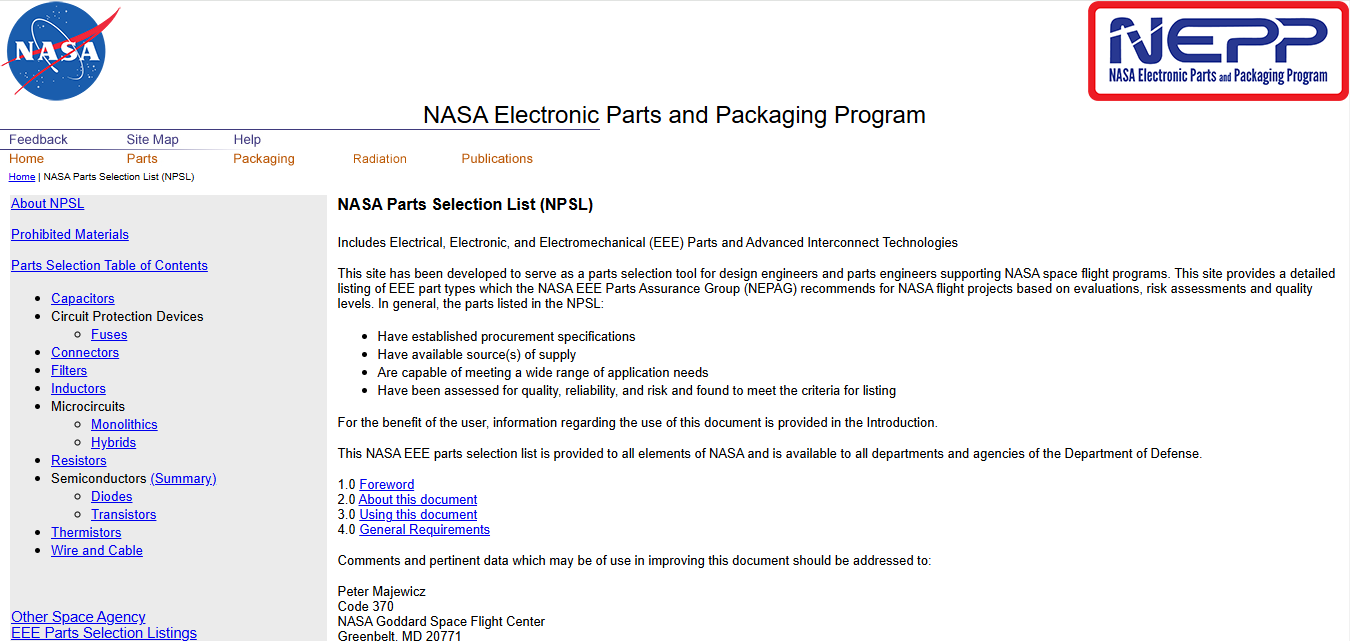
\includegraphics[width=\linewidth]{images/NPSL.png}
    \label{fig:npsl}
    \fonte{NASA, 2016.}
\end{figure}

No caso da ECSS-Q-ST-60C, há uma organização dos componentes em classes, balanceando níveis de risco e confiabilidade. Essa norma indica, de forma geral, os requisitos de seleção e uso de componentes para projetos espaciais da ESA, o que será crucial para realização desse trabalho.

Além disso, ao entender o estado da arte dos OBDHs projetados para nanossatélites, pode-se também escolher componentes por meio da herança de voo, ou seja, escolhendo componentes que já estiveram em missões semelhantes ou mais críticas.

Por fim, em alguns casos de circuitos mais complexos, os requisitos impedem que se tenha herança de voo ou que os componentes estejam presentes em uma base de dados da NASA ou da ESA. Nesse caso, será seguido cada recomendação do fabricante do circuito integrado crítico (como um SoC ou uma memória). 

Com isso, é possível começar a projetar o \textit{hardware} do OBDH, utilizando as diretrizes citadas e as heranças de voo, tomando como base os projetos citados, escolhendo os componentes e respeitando os requisitos impostos.



% Citação: 
% https://sci-hub.se/10.1109/jproc.2018.2802438
 


% ----------------------------------------------------------
\chapter{Arquitetura}
% ----------------------------------------------------------

Após estudar os desdobramentos dos efeitos de órbita baixa e entender o que é necessário para se realizar um projeto confiável de computador de bordo de um nanossatélite através de projetos anteriores, foi necessária a compreensão dos requisitos de projeto. Com isso, foram escolhidos os componentes principais da placa, propondo-se uma arquitetura para o sistema para um \textit{hardware} confiável, robusto e versátil.  

\section{Requisitos de Projeto}

Como dito, foi preciso entender os requisitos impostos para o OBDH da terceira geração do SpaceLab. Com base nas necessidades levantadas para o laboratório nos próximos projetos e na revisão do estado da arte, são apresentados na Tabela \ref{tab:Tab_Req} os requisitos gerais do projeto, em conjunto com a \textit{rationale} e com o método de verificação (NASA Product Verification, 2024). Outro ponto importante a ser considerado seriam as revisões de projeto, que não foram consideradas nesse trabalho.

\begin{longtable}{@{}>{\centering}p{1.5cm}p{4cm}p{4cm}p{4.7cm}@{}}
    \centering
	\ABNTEXfontereduzida
	\label{tab:Tab_Req}\tabularnewline
	\caption{Requisitos do OBDH da terceira geração do SpaceLab.}\tabularnewline
	%\begin{tabular}{@{}p{2cm}p{2cm}p{2cm}p{2cm}p{2cm}p{2cm}p{3cm}@{}}
	\hline
	\multicolumn{1}{c}{\textbf{Índice}} & \multicolumn{1}{c}{\textbf{Descrição}} & \multicolumn{1}{c}{\textbf{Rationale}} & \multicolumn{1}{c}{\textbf{Método de Verificação}} \tabularnewline
        \hline
        1 & O módulo OBDH deve ser compatível com o padrão CubeSat & Assegura compatibilidade com outros satélites desenvolvidos no SpaceLab & Inspeção \tabularnewline
        
       \hline
        2 & O módulo OBDH deve operar corretamente entre -40°C e 85°C & Para operar com segurança em um ambiente LEO & Teste e Análise \tabularnewline

       \hline
       3 & O módulo OBDH deve possuir um processador capaz de usar um sistema RTOS & Para gerenciar e coordenar operações dentro e fora do módulo, sendo capaz de realizar tarefas complexas definidas pela equipe  & Inspeção \tabularnewline

       \hline
        4 & O módulo OBDH deve possuir uma memória DDR com capacidade de 512Mb (preferencialmente com ECC)  & Memória suficiente para operações do OBDH e armazenamento de dados  & Inspeção\tabularnewline

        \hline
       5 & O módulo OBDH deve possuir uma memória FRAM para armazenar parâmetros de configuração & Provê memória não-volátil e duradoura, menos sucetível à radiação & Inspeção \tabularnewline 

        \hline
        6 & O módulo OBDH deve possuir uma memória Flash para armazenar dados do satélite (preferencialmente com ECC) & Para armazenar dados & Inspeção \tabularnewline 

        \hline
       7 & O módulo OBDH deve possuir um WDT (\textit{Watchdog Timer}) para reiniciar o processador em caso de falha de \textit{software} & Reinicia automaticamente o processador caso haja a falha  & Teste \tabularnewline

        \hline
       8 & O módulo OBDH deve possuir sensores de medição de tensão e corrente em seus barramentos de alimentação & Para monitoramento de potência consumida & Inspeção \tabularnewline

        \hline
      9 &  O módulo OBDH deve possuir proteção de sobrecorrente (20\% acima do valor nominal) & Para proteção contra \textit{latch-up}  & Análise \tabularnewline

        \hline
        10 & O módulo OBDH deve possuir um giroscópio para medição de velocidade angular & Para permitir controle de atitude ativo do satélite  & Inspeção \tabularnewline 

       \hline
       11 & O módulo OBDH deve possuir um magnetômetro & Para permitir controle de atitude ativo do satélite  & Inspeção \tabularnewline

        \hline
        12 & O módulo OBDH deve possuir uma interface RS-422 para transmissão de mensagens de \textit{debug/log} e receber parâmetros de configuração & Comunicação de longa distância com maior imunidade ao ruído e maior taxa de dados  & Teste \tabularnewline

       \hline
       13 & O módulo OBDH deve possuir uma interface CAN para receber e transmitir comandos e dados & Para comunicação robusta e com suporte a múltiplos subsistemas do CubeSat  & Inspeção \tabularnewline

        \hline
        14 & O módulo OBDH deve possuir uma interface acessível externamente para programação do microcontrolador & Para o módulo ser facilmente programado pelo time  & Inspeção \tabularnewline

        \hline
        15 & O módulo OBDH deve possuir uma interface para um barramento de expansão & Para prover suporte a outras interfaces e periféricos  & Inspeção \tabularnewline

        \hline
       16 & O módulo OBDH deve possuir um sensor de temperatura com precisão menor ou igual a 1°C & Para monitorar a temperatura de operação & Inspeção\tabularnewline

        \hline
       17 & O módulo OBDH deve possuir uma interface RS-485 para receber e transmitir comandos e dados  & Para comunicação robusta e com suporte a múltiplos subsistemas do CubeSat & Inspeção \tabularnewline
       \hline
\end{longtable}
{\fonte{Elaboração própria.}}

Com as definições apresentadas na Tabela \ref{tab:Tab_Req}, foi então necessária a definição da arquitetura do hardware, ou seja, os componentes e sua interconexões, bem como as interfaces de comunicação e saídas necessárias.

\section{Arquitetura Proposta}

A partir dos requisitos, o primeiro passo foi definir de forma geral como seria o funcionamento do \textit{hardware} do projeto. Na Figura \ref{fig:arq_geral}, pode-se verificar um esquema inicial de proposta de arquitetura, usando os pontos descritos anteriormente.

\begin{figure}[H]
    \centering
    \caption{Esquema geral de arquitetura.}
    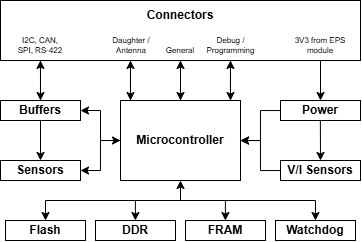
\includegraphics[scale=1.2]{images/arquitetura geral.png}
    \label{fig:arq_geral}
    \fonte{Elaboração própria.}
\end{figure}

Como podemos verificar, o processador será crucial e deverá ter pinos suficientes para interface com todas as memórias, sensores e para se comunicar com os outros módulos do CubeSat. Além disso, a parte dos circuitos dedicados aos barramentos de alimentação deverá ser cuidadosamente estudada, para que seja corretamente dimensionado de acordo com o consumo de potência estimado. A escolha de cada componente será descrita nas seções a seguir, respeitando sempre os seguintes critérios:

\begin{itemize}
	\item O componente deve funcionar corretamente nas temperaturas entre -40°C e 85°C;
	\item Circuitos integrados devem possuir herança de voo sempre que possível;
	\item Caso o circuito integrado necessite de um circuito específico, o mesmo deve conter itens preferencialmente dispostos na ECSS-Q-ST-60C, na NPSL ou similar aos mesmos, especialmente componentes discretos (capacitores, resistores, indutores, diodos, transistores, entre outros);
\end{itemize}

\subsection{Microcontrolador}

Como visto na Tabela \ref{tab:Tab_Missoes}, a fabricante com maior herança de voo estudada é a Xilinx, em especial os chips da família Zynq 7000, que são SoCs. Após um estudo próprio, o SoC Zynq 7030 se mostrou mais adequado pelas seguintes características:

\begin{itemize}
	\item Foi usado em missões extensivas em pequenos satélites (GomSpace, 2024), ou seja, possui herança de voo em missões similares em LEO e em CubeSats;
	\item Possui um envelopamento com 484 pinos, suficiente para prover as conexões necessárias para todas as interfaces requeridas (UG865, 2021);
	\item Capaz de rodar um sistema operacional Linux (KADI et al.,2013);
	\item Por ser um SoC, possui alta adaptabilidade e flexibilidade, disponibilizando no mesmo chip uma FPGA e um microprocessador, denominados respectivamente de PL (\textit{Programmable Logic}) e PS (\textit{Processing System});
\end{itemize}

\subsection{Memórias}

As memórias serão necessárias para realizar operações, armazenar dados externos e internos e armazenar parâmetros de configuração do OBDH e de outros subsistemas do CubeSat. Para cada uma dessas funções uma memória diferente é necessária, seguindo suas características principais, sendo elas: tempo de acesso, tamanho do armazenamento e volatilidade.

\subsubsection{Memórias voláteis}

Partindo dos requisitos de projeto, bem como do esforço de se obter um \textit{hardware} capaz de rodar um sistema Linux, a principal opção se tornou as memórias do tipo DDR (\textit{Double Data Rate}), que utilizam ambas a borda de subida e de descida para transferência de dados para atingir o dobro de largura de banda de uma memória com SDR (\textit{Single Data Rate}) para uma mesma frequência de relógio (JEDEC, 2008). Essa relação pode ser ilustrada pela Figura \ref{fig:sdrvsddr}, onde pode-se verificar a transferência de dados do sinal DQ em relação ao sinal de relógio (bCLK e CLK) para SDR e DDR.

\begin{figure}[H]
    \centering
    \caption{Comparação entre DDR e SDR.}
    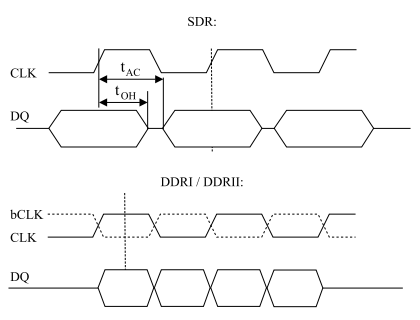
\includegraphics[scale=1]{images/ddrsdr.png}
    \label{fig:sdrvsddr}
    \fonte{KLEHN E BROX, 2003.}
\end{figure}
 
Por essa razão, bem como pelo fato de que para rodar um sistema operacional complexo (seja ele RTOS ou Linux) existam requisitos de memória RAM, foi escolhida uma memória do tipo DDR3, com capacidade de 2Gb (256 MB) e frequência de operação de 800 MHz.

\subsubsection{Memórias não voláteis}

No caso das memórias não voláteis, é necessária uma atenção especial ao tipo de dado que será armazenado em cada uma delas. Para o caso de dados críticos, é preciso de uma memória que possua alta resistência aos efeitos da radiação, mantendo-se um compromisso com os tempos de escrita e leitura. Por sua vez, para dados de inicialização são mais críticos os tempos de leitura, enquanto para uma memória de dados mais gerais, o importante é o armazenamento total. Por meio desses critérios, foi possível avaliar, por meio da Tabela \ref{tab:memnvol}, o tipo de memória ideal para cada caso, considerando o número máximo de ciclos de leitura e escrita de cada tipo de memória.

\begin{table}[H]
	\ABNTEXfontereduzida
	\caption{\label{tab:memnvol}Tabela comparativa de memórias não voláteis.}
	%\begin{tabular}{@{}p{2cm}p{2cm}p{2cm}p{2cm}p{2cm}p{2cm}p{3cm}@{}}
    \centering
    \begin{tabular}{@{} >{\centering}p{2cm} >{\centering}p{3cm} >{\centering}p{3cm} >{\centering}p{3cm}>{\centering}p{3cm} @{}}
    
		\toprule
		\textbf{Memória} & \textbf{Tempo de leitura/escrita} & \textbf{Tolerância à radiação} & \textbf{Armazenamento máximo} & \textbf{Ciclos de escrita / apagamento} \tabularnewline 
        \midrule
        Flash NOR & \textasciitilde{} 1$\mu$s & Ruim & \textasciitilde{} 1 Gb & \textbf{$10^5$} \tabularnewline
        
        \midrule
        Flash NAND & \textasciitilde{} 100 $\mu$s & Ruim &\textasciitilde{} 1 Tb & \textbf{$10^5$} \tabularnewline 

        \midrule
        FRAM & \textasciitilde{} 50 ns & Boa & \textasciitilde{} 1 Mb & \textbf{$10^{15}$}  \tabularnewline 
        
        \bottomrule
	\end{tabular}
	\fonte{Elaboração própria com base em (GERARDIN E PACCAGNELLA, 2010) e (BOUKHOBZA E OLIVIER, 2017).}
\end{table}

Com isso, foi então escolhida uma FRAM para armazenar dados críticos, uma Flash NAND para armazenamento de dados gerais e uma Flash NOR para armazenar o boot do sistema operacional no SoC.

\subsection{Conversores DC-DC}
Nos sistemas CubeSat do SpaceLab da UFSC, o módulo responsável pelo fornecimento de potência é o chamado EPS (MARCELINO, 2024). A partir disso, partindo do pressuposto que haverá uma tensão fornecida de 3,3 V, pode-se inferir a cascata dos barramentos de alimentação a partir do mesmo. Para o caso do Zynq e da memória DDR3, circuitos integrados são necessários para gerar as seguintes tensões: 

\begin{itemize}
	\item Zynq: 1 V e 1,8 V; 
	\item DDR3L: 1,35 V e 0,675 V.
\end{itemize}

Todos os demais periféricos devem aceitar uma tensão de alimentação de 3,3 V. Outro ponto importante são os circuitos de proteção contra \textit{latch-up}, um efeito similar a um curto-circuito na trilha de alimentação de circuitos CMOS (AN-600, 1989). Essa proteção é essencial, pois ao ocorrer, gera um consumo elevado de corrente e consequentemente tem potencial de gerar efeitos e falhas catastróficas (ECSS, 2018). No caso desse projeto, será utilizado o LTC4361, anteriormente usado em outras PCBs do SpaceLab, como o Payload HARSH (MATTOS, 2020). 

Na Figura \ref{fig:diapower}, está esquematizado o sistema de potência proposto.

\begin{figure}[H]
    \centering
    \caption{Sistema de potência proposto.}
    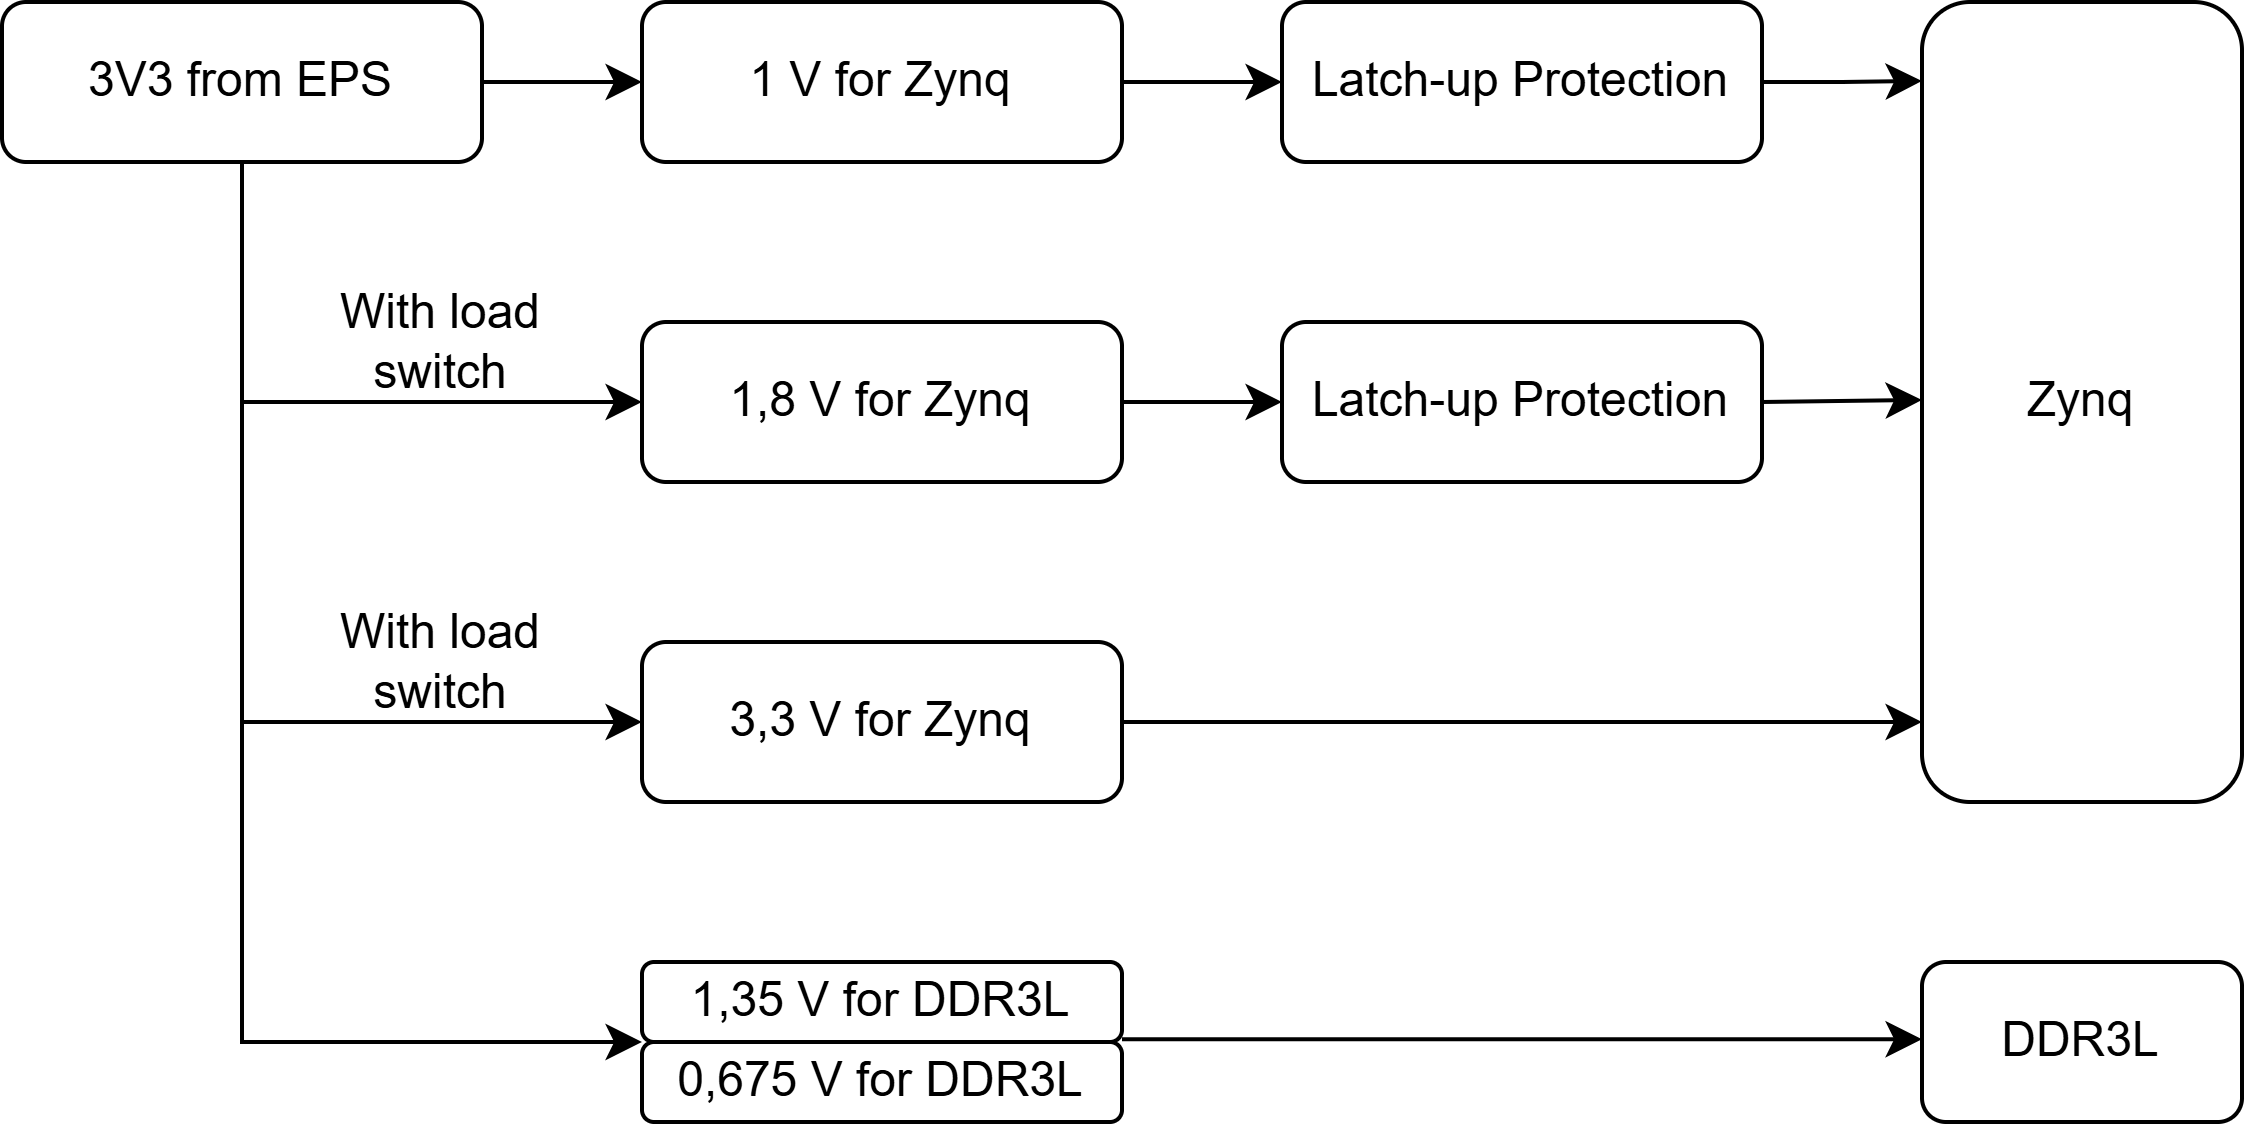
\includegraphics[scale=1]{images/diapower.png}
    \label{fig:diapower}
    \fonte{Elaboração própria.}
\end{figure}

\subsection{Sensores e Periféricos}
Como dito nos requisitos, alguns sensores precisam estar presentes no OBDH. Entre eles:

\begin{itemize}
	\item Um monitor de tensão, para todas os barramentos de alimentação importantes do sistema;
	\item Um sensor de corrente para o barramento de alimentação principal do módulo;
	\item Um giroscópio para medir a velocidade angular em órbita;
	\item Um magnetômetro para medição do campo magnético da Terra em órbita;
	\item Um WDT para reiniciar o sistema em caso de falha de software;
	\item Um sensor de temperatura para o SoC e um para a região das memórias na PCB;
\end{itemize}

\section{Visualização da Arquitetura Proposta}

Depois das decisões tomadas, foi possível montar um diagrama, apresentado na Figura \ref{fig:arq}, que mostra cada circuito do computador de bordo. Aqui, por simplicidade, foram suprimidos os circuitos da parte de potência do módulo.

\begin{figure}[H]
    \centering
    \caption{Arquitetura proposta para o OBDH.}
    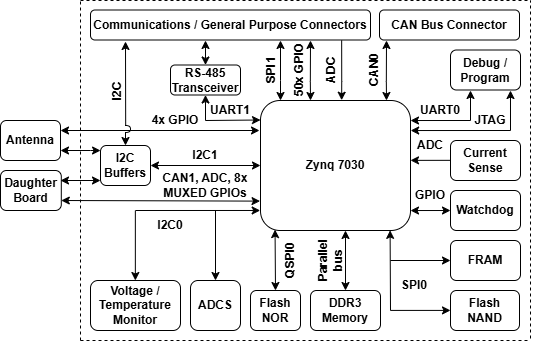
\includegraphics[scale=1]{images/arquitetura final.png}
    \label{fig:arq}
    \fonte{Elaboração própria.}
\end{figure}

Também foram levadas em consideração as interfaces disponibilizadas pelo SoC, os componentes escolhidos e os conectores necessários. Os componentes escolhidos se encontram na Tabela \ref{tab:componentes}, conjuntamente com as interfaces requeridas para cada um, suas tensões de alimentação e suas correntes máximas no terminal de alimentação, no pior caso especificado pelo fabricante.

\begin{table}[H]
	\ABNTEXfontereduzida
	\caption{\label{tab:componentes}Informações sobre os componentes escolhidos.}
	%\begin{tabular}{@{}p{2cm}p{2cm}p{2cm}p{2cm}p{2cm}p{2cm}p{3cm}@{}}
    \centering
    \begin{tabular}{@{} >{\centering}p{2cm} >{\centering}p{4cm} >{\centering}p{2cm} >{\centering}p{3cm}>{\centering}p{3cm} @{}}
    
		\toprule
		\textbf{Componente} & \textbf{Número do Fabricante} & \textbf{Interface} & \textbf{Tensão de Alimentação} & \textbf{Corrente máxima} \tabularnewline 
        \midrule
        FRAM & CY15B104QN-50SXI & SPI & 3,3 V & 3,7 mA \tabularnewline
        
        \midrule
        Flash NOR & MT25QL128ABB1ESE-0AUT & QSPI & 3,3 V & 35 mA \tabularnewline 

        \midrule
        Flash NAND & MT29F1G01ABAFDSF-AAT:F & SPI & 3,3 V & 55 mA \tabularnewline 

        \midrule
        DDR3L & MT41K256M8DA-125:K & Paralela & 1,35 V & 182 mA \tabularnewline 

        \midrule
        WDT & TPS3823-33QDBVRQ1 & - & 3,3 V & 10 mA \tabularnewline 

        \midrule
        Monitor de Temperatura e Tensão & LTC2991IMS\#TRPBF & I2C & 3,3 V &  1,5 mA \tabularnewline 

        \midrule
        Sensor de Corrente & INA180A2IDBVR & - & 3,3 V & 1 mA \tabularnewline 

        \midrule
        Giroscópio & A3G4250D & I2C & 3,3 V & 7 mA \tabularnewline 

        \midrule
        Magnetômetro & MMC5983MA & I2C & 3,3 V & 0,45 mA \tabularnewline 

        \midrule
        Buffer I2C & TCA4311ADR & I2C & 3,3 V & 7 mA \tabularnewline 

        \midrule
        Transceptor CAN & TCAN330D & CAN & 3,3 V & 60 mA \tabularnewline 

        \midrule
        Transceptor RS-485 & THVD1451DR & Serial & 3,3 V & 3 mA \tabularnewline 

        \midrule
        Conversor DC-DC & TPS82085SILR & - & 3,3 V & - \tabularnewline 

        \midrule
        Conversor DC-DC para DDR3 & TPS51200DRCR & - & 3,3 V & 1 mA \tabularnewline 

        \midrule
        \textit{Load Switch} & TPS22920YZPR & - & 3,3 V & 0,2 mA \tabularnewline 
        
        \midrule
        Proteção contra \textit{Latch-up} & LTC4361 & - & - & - \tabularnewline 

        \bottomrule
	\end{tabular}
	\fonte{Elaboração própria com base nos Datasheets de cada componente.}
\end{table}

\subsection{Estimativa de Potência Consumida}

A fim de garantir o funcionamento correto dos conversores DC-DC e seus respectivos periféricos, foi necessária uma estimativa da potência total consumida por todas as tensões disponíveis no módulo. Para isso, foi utilizada a Tabela \ref{tab:componentes}, bem como o datasheet de cada componente, com a corrente máxima do barramento de alimentação (levando-se em consideração as correntes de chaveamento e quiescentes). No caso do SoC, sua fabricante disponibiliza uma planilha (XPE, 2019) para estimativas de potência em cada tensão de alimentação. 

Com isso, foram obtidos os valores da Tabela \ref{tab:estpoww}, considerando uma eficiência de conversão de 85\% (TPS82085, 2019), já incluindo as estimativas de potência e os piores casos descritos anteriormente. 

\begin{table}[H]
	\ABNTEXfontereduzida
	\caption{\label{tab:estpoww}Estimativas de potência consumida no pior caso.}
	%\begin{tabular}{@{}p{2cm}p{2cm}p{2cm}p{2cm}p{2cm}p{2cm}p{3cm}@{}}
    \centering
    \begin{tabular}{@{} >{\centering}p{2cm} >{\centering}p{4cm} >{\centering}p{4cm} >{\centering}p{4cm}@{}}
    
		\toprule
		\textbf{Tensão [V]} & \textbf{Potência Dissipada [W]} & \textbf{Potência dissipada na tensão de 3,3 V [W]} & \textbf{Corrente máxima da trilha [A]} \tabularnewline 
        \midrule
         1,00 & 2,20 & 2,59 & 2,20 \tabularnewline
        
        \midrule
        1,35 & 0,25 & 0,29 & 0,18 \tabularnewline 

        \midrule
        1,80 & 0,63 & 0,74 & 0,35 \tabularnewline

        \midrule
        3,3 & 3,88 & - & -  \tabularnewline        

        \bottomrule
	\end{tabular}
	\fonte{Elaboração própria.}
\end{table}

Através dessas estimativas, pode-se inferir que o sistema de potência proposto suporta os componentes escolhidos e suas tensões e variações, mesmo quando se considera o pior caso, totalizando uma potência total consumida de 7,5 W, ou seja, 2,27 A no barramento proveniente do EPS. Agora, partindo do mesmo percentual de eficiência, é considerado um caso típico, apresentado na Tabela \ref{tab:estpow}. 

\begin{table}[H]
	\ABNTEXfontereduzida
	\caption{\label{tab:estpow}Estimativas de potência consumida no caso típico.}
	%\begin{tabular}{@{}p{2cm}p{2cm}p{2cm}p{2cm}p{2cm}p{2cm}p{3cm}@{}}
    \centering
    \begin{tabular}{@{} >{\centering}p{2cm} >{\centering}p{4cm} >{\centering}p{4cm} >{\centering}p{4cm}@{}}
    
		\toprule
		\textbf{Tensão [V]} & \textbf{Potência Dissipada [W]} & \textbf{Potência dissipada na tensão de 3,3 V [W]} & \textbf{Corrente típica da trilha [A]} \tabularnewline 
        \midrule
         1,00 & 0,67 & 0,79 & 0,67 \tabularnewline
        
        \midrule
        1,35 & 0,127 & 0,15 & 0,13 \tabularnewline 

        \midrule
        1,80 & 0,51 & 0,60 & 0,28 \tabularnewline

        \midrule
        3,3 & 3,2 & - & -  \tabularnewline        

        \bottomrule
	\end{tabular}
	\fonte{Elaboração própria.}
\end{table}

Com esses resultados, já estão sendo considerados os superdimensionamentos dos conversores de potência. Nesse caso, o consumo típico total é próximo de 4,7 W, ou seja, com uma corrente de 1,4 A no barramento proveniente do EPS. Mesmo assim, é possível adotar técnicas no firmware para diminuir o consumo mesmo no caso típico, ativando e desativando entradas e saídas conforme o necessário, visto que essa tabela pressupõe que todos os componentes estão em funcionamento ao mesmo tempo, incluindo memórias e transceptores.
% ----------------------------------------------------------
\chapter{Desenvolvimento do Projeto}
% ----------------------------------------------------------

Depois das definições apresentadas e da escolha de componentes apresentada na seção anterior, foi possível construir um esquemático elétrico, que esquematiza a PCB do OBDH. Nesse capítulo, discutir-se-á circuitos específicos mais relevantes do projeto, usando o esquemático pronto, que se encontra no Apêndice A. O \textit{software} utilizado para construção desse esquemático foi o Altium Designer (versão 24.4.1).

\section{Conversores de Potência}

Partindo do princípio que o módulo EPS da terceira geração de módulos do SpaceLab será capaz de fornecer 3,3 V para o OBDH, foi proposta uma cascata de potência descrita na Figura \ref{fig:power}. Nela, são suprimidos os circuitos de proteção que serão descritos posteriormente.

\begin{figure}[H]
    \centering
    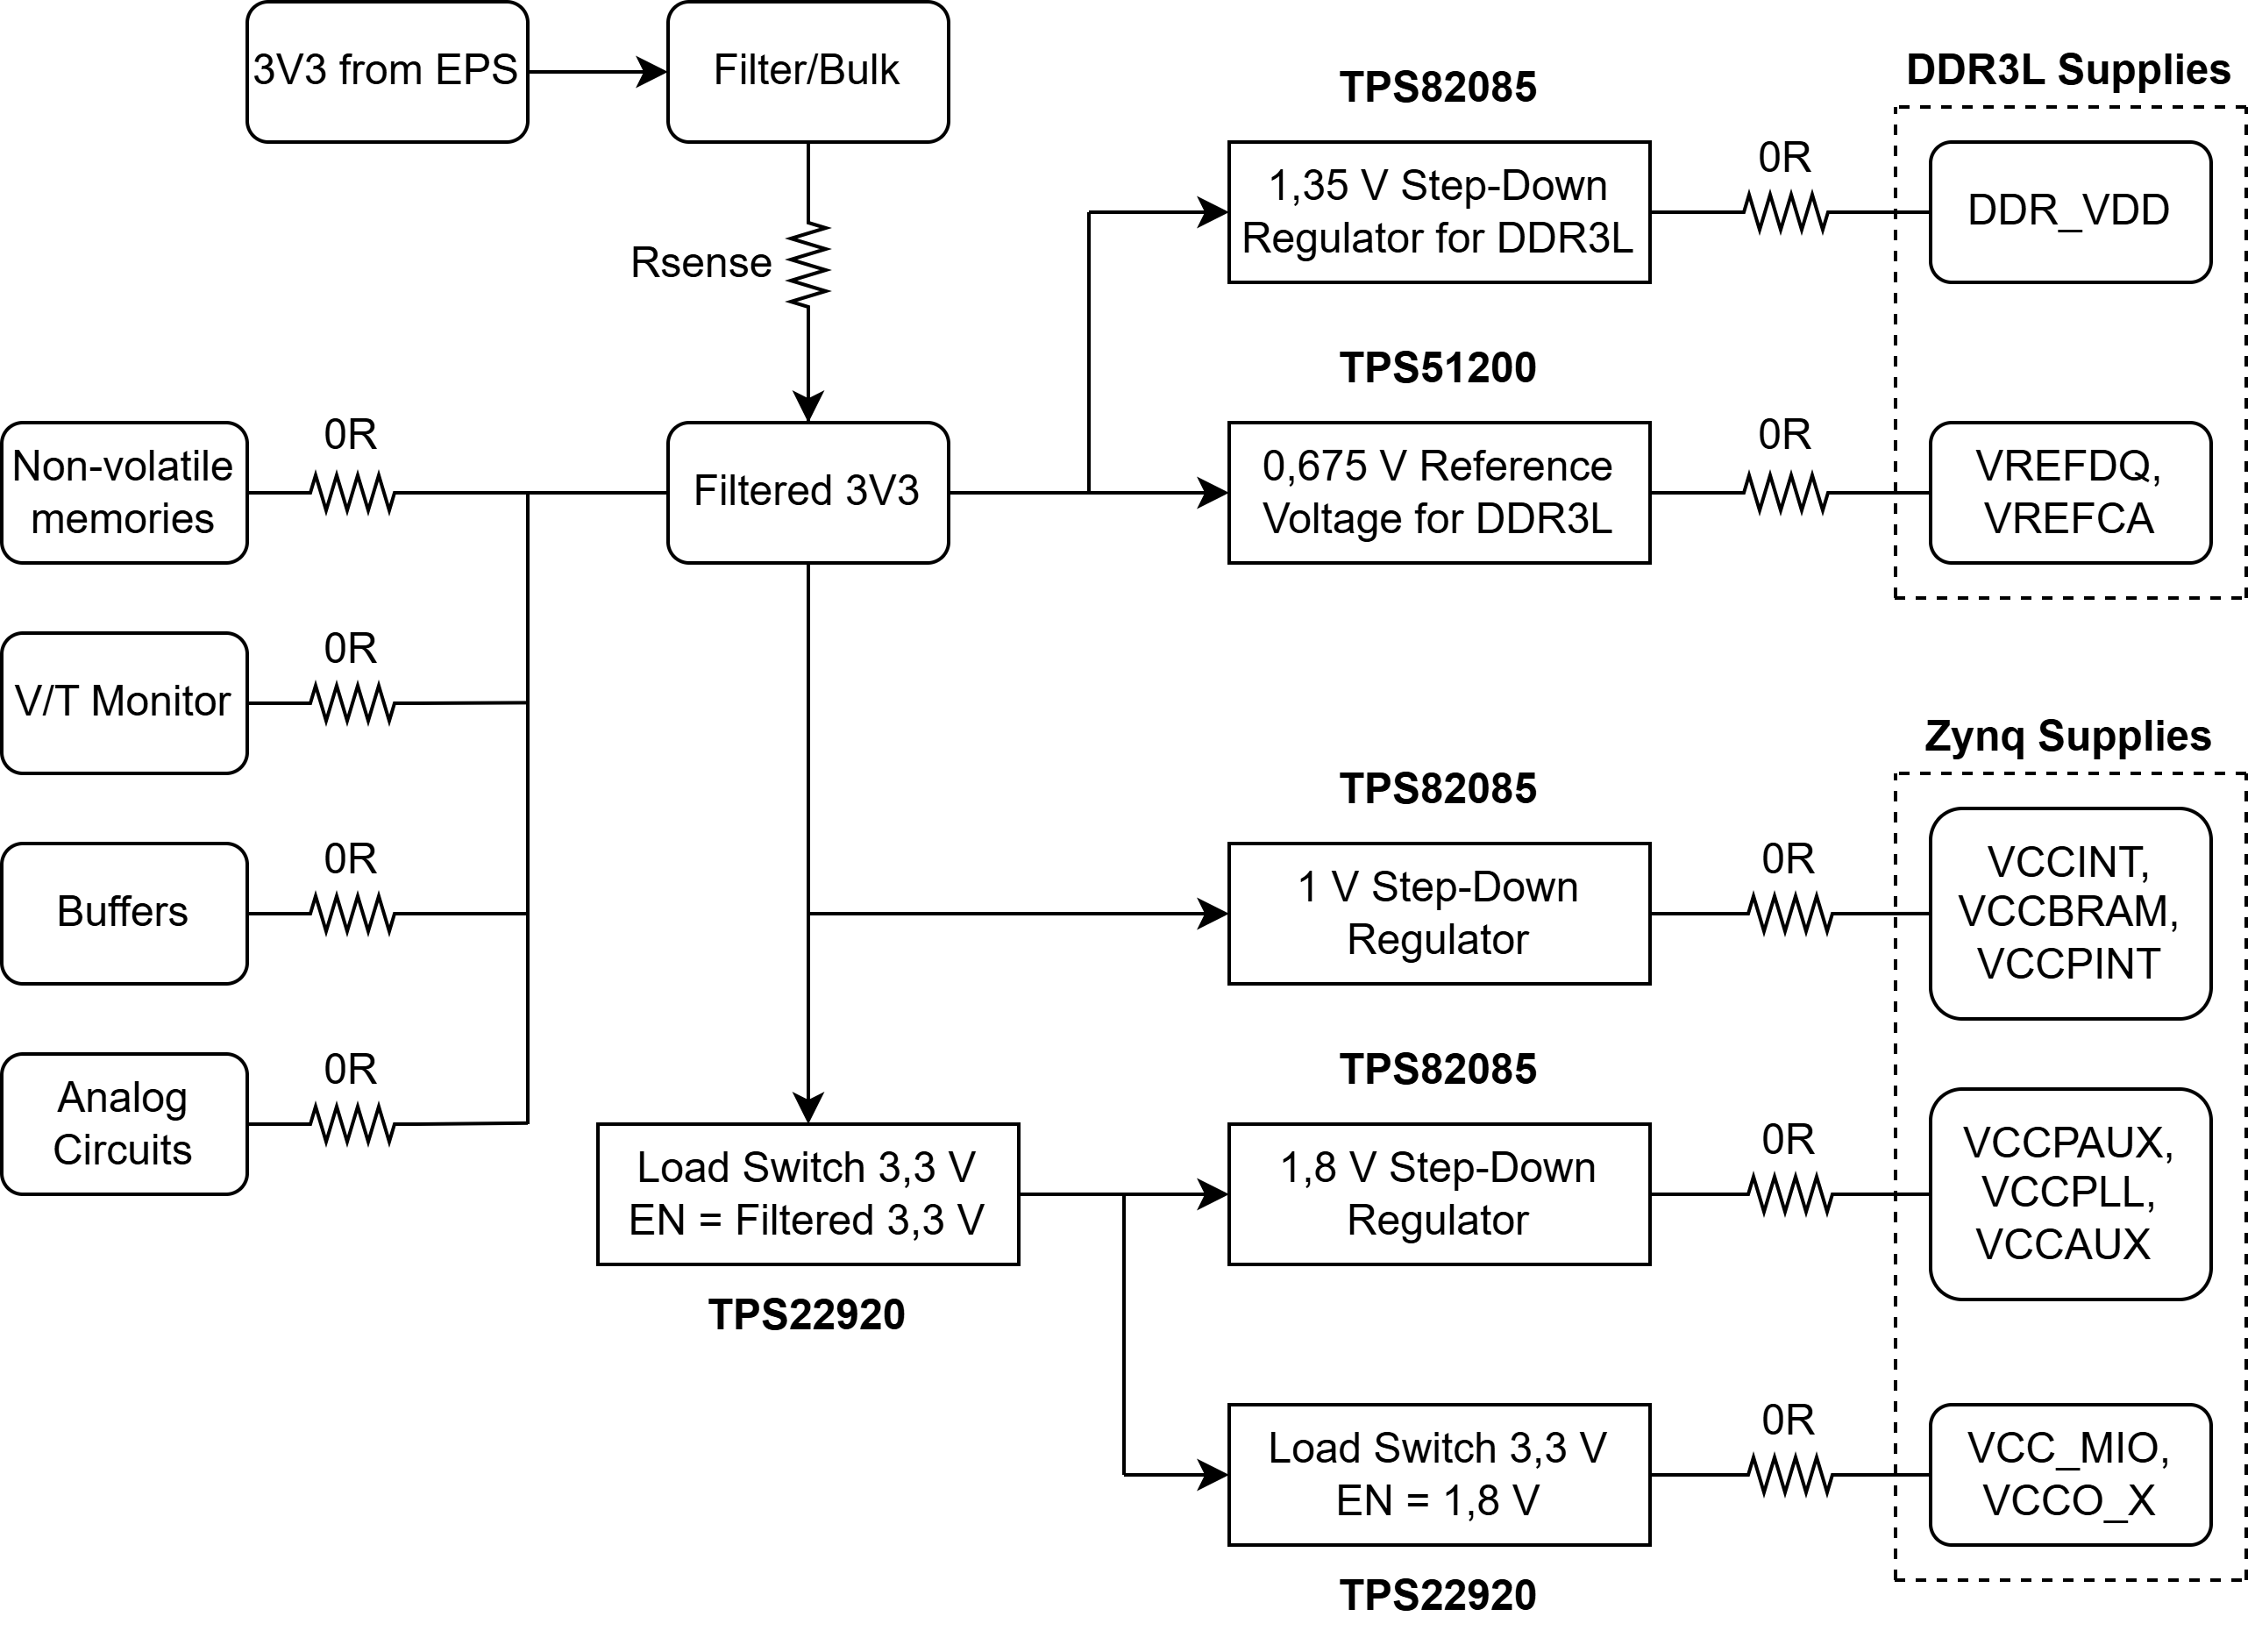
\includegraphics[scale=0.8]{images/Power_system.png}
    \caption{Cascata de potência proposta.}
    \label{fig:power}
    \fonte{Elaboração própria.}
\end{figure}

\subsection{Filtro de Entrada}

Costumeiramente, a entrada de tensão de uma placa robusta deve ser filtrada, principalmente devido às flutuações do ruído conduzido de outros subsistemas do satélite, caracterizando o fenômeno de Interferência Eletromagnética (EMI), esquematizado na Figura \ref{fig:emi}.

\begin{figure}[H]
    \centering
    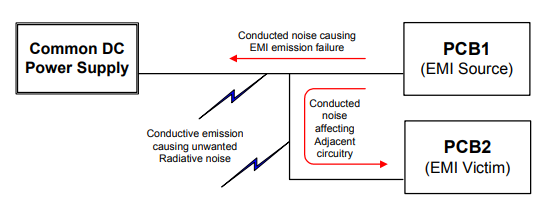
\includegraphics[scale=1]{images/EMI noise.png}
    \caption{Interferência com ruído conduzido.}
    \label{fig:emi}
    \fonte{SOH et al., 2010.}
\end{figure}

Além disso, também foi necessária a inclusão de um diodo Zener em paralelo à entrada, servindo como um elemento extra de proteção contra perturbações e transientes (CADENCE, 2023). Outra característica explorada foi a colocação de capacitores em paralelo, a fim de reduzir sua resistência em série equivalente (ESR) e sua indutância série (SARJEANT, 1990).  O filtro proposto está disposto na Figura \ref{fig:FILTRO}.  Além disso, sua magnitude e fase simuladas estão dispostas na Figura \ref{fig:filtrof}, utilizando o software LTSPICE XVII.

\begin{figure}[H]
    \centering
    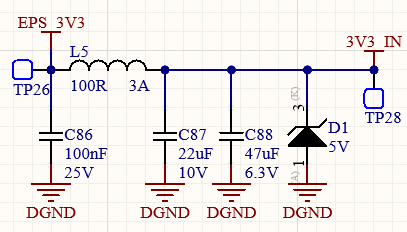
\includegraphics[scale=1]{images/FILTRO.png}
    \caption{Filtro proposto.}
    \label{fig:FILTRO}
    \fonte{Elaboração própria.}
\end{figure}

\begin{figure}[H]
    \centering
    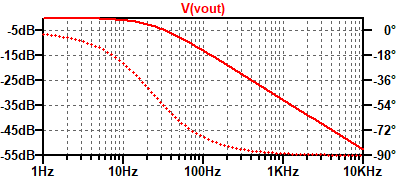
\includegraphics[scale=1]{images/filtrof.png}
    \caption{Simulação de magnitude e fase em função da frequência para o filtro proposto.}
    \label{fig:filtrof}
    \fonte{Elaboração própria.}
\end{figure}

\subsection{Cascata de potência}

Devido à escolha do SoC e da memória DDR3, foi necessária a definição de uma cascata de potência, levando-se em consideração os requisitos de (UG585, 2023), que descreve o sequenciamento das tensões para o menor consumo de potência e para garantir a integridade do fusível interno do SoC. Dessa forma, como pode-se ver na Figura \ref{fig:power}, são usados os denominados \textit{load switches}, a fim de garantir o sequenciamento descrito e garantir uma proteção efetiva contra sobrecorrente (MAK, 2018). 

O primeiro regulador, que gera a tensão de 1 V, apresentado na Figura \ref{fig:1vsupp}, é o primeiro da cascata. Seu divisor de tensão de saída foi calculado conforme (TPS82085, 2019):

\begin{equation}
	V_{out} = 0,8 * (1 + R_1/R_2) = 0,8 * (1+ 37,4k/150k) = 0,999 V
\end{equation} 

\begin{figure}[H]
    \centering
    \includegraphics[scale=0.8]{images/1vsupp.png}
    \caption{Regulador de tensão de 1 V.}
    \label{fig:1vsupp}
    \fonte{Elaboração própria com base no circuito apresentado pelo fabricante.}
\end{figure}

Também foi possível montar seu circuito de proteção de sobrecorrente, disposto na Figura \ref{fig:1vocp}. Seu resistor de entrada, que escolhe o limiar de corrente permitido, foi caculado conforme (LTC4361, 2018), considerando uma corrente 20\% superior à máxima calculada (na Tabela \ref{tab:estpow}):

\begin{equation}
	R_{sense} = 50 mV / I_{max} =50 / 2,63 = 19,01 m\Omega
\end{equation} 

\begin{figure}[H]
    \centering
    \includegraphics[scale=1]{images/1vocp.png}
    \caption{Proteção contra \textit{latch-up} para a tensão de 1 V.}
    \label{fig:1vocp}
    \fonte{Elaboração própria com base no circuito apresentado pelo fabricante.}
\end{figure}

Depois disso, para seguir com o sequenciamento requerido pelo SoC, precisa-se de um circuito de chaveamento de carga, apresentado na Figura \ref{fig:sw1}. Seu circuito é baseado no sugerido por (TPS22920, 2016), com sua ativação o sendo realizada pela própria tensão de 3,3 V.

\begin{figure}[H]
    \centering
    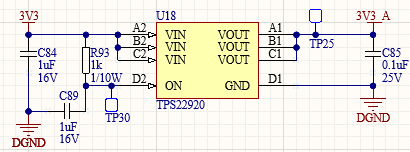
\includegraphics[scale=1]{images/sw1.png}
    \caption{Circuito de \textit{Load switch} para a tensão de 1,8 V.}
    \label{fig:sw1}
    \fonte{Elaboração própria com base no circuito apresentado pelo fabricante.}
\end{figure}

Analogamente, para a tensão de 1,8 V, são necessários ambos um conversor e um circuito de proteção. Estes estão dispostos respectivamente nas Figuras \ref{fig:1v8supp} e \ref{fig:1v8ocp} a seguir, conjuntamente com suas equações (3) e (4) para obtenção das resistências requeridas, usando a mesma margem de 20\% de corrente máxima. 

\begin{equation}
	V_{out} = 0,8 * (1 + R_1/R_2) = 0,8 * (1+ 110k/88,7k) = 1,792 V
\end{equation} 

\begin{figure}[H]
    \centering
    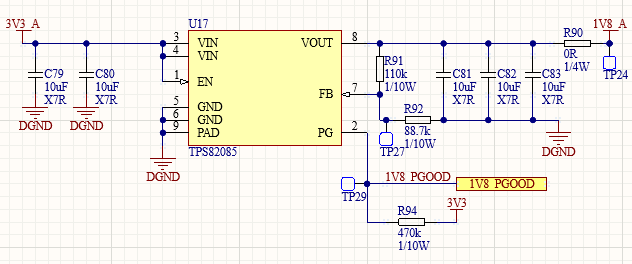
\includegraphics[scale=0.8]{images/1v8supp.png}
    \caption{Regulador de tensão de 1,8 V.}
    \label{fig:1v8supp}
    \fonte{Elaboração própria com base no circuito apresentado pelo fabricante.}
\end{figure}

\begin{equation}
	R_{sense} = 50 mV / I_{max} =50 / 0,5 = 100 m\Omega
\end{equation} 

\begin{figure}[H]
    \centering
    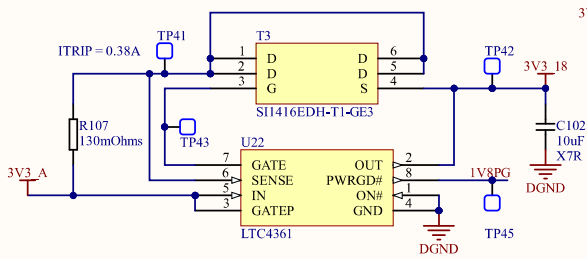
\includegraphics[scale=1]{images/1v8ocp.png}
    \caption{Proteção contra \textit{latch-up} para a tensão de 1,8 V.}
    \label{fig:1v8ocp}
    \fonte{Elaboração própria com base no circuito apresentado pelo fabricante.}
\end{figure}

Por fim, para ligar a tensão de 3,3 V fornecida para o SoC, é necessário um último circuito de chaveamento, dessa vez com sua ativação realizada pela tensão de 1,8 V, como mostra a Figura \ref{fig:sw2}.

\begin{figure}[H]
    \centering
    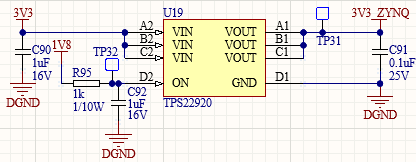
\includegraphics[scale=1]{images/sw2.png}
    \caption{Circuito de \textit{Load switch} para a tensão de 3,3 V do SoC.}
    \label{fig:sw2}
    \fonte{Elaboração própria com base no circuito apresentado pelo fabricante.}
\end{figure}

Paralelamente, para a memória DDR3L, são necessários um conversor para a alimentação, de 1,35 V, e um conversor para a tensão de referência e de terminação. Esses circuitos estão dispostos respectivamente nas Figuras \ref{fig:1v35supp} e \ref{fig:1v35ref}.

\begin{equation}
	V_{out} = 0,8 * (1 + R_1/R_2) = 0,8 * (1+ 47k/68k) = 1,353 V
\end{equation} 

\begin{figure}[H]
    \centering
    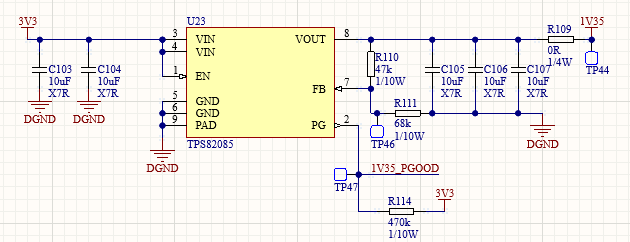
\includegraphics[scale=0.8]{images/1v35supp.png}
    \caption{Regulador de tensão de 1,35 V.}
    \label{fig:1v35supp}
    \fonte{Elaboração própria com base no circuito apresentado pelo fabricante.}
\end{figure}

\begin{figure}[H]
    \centering
    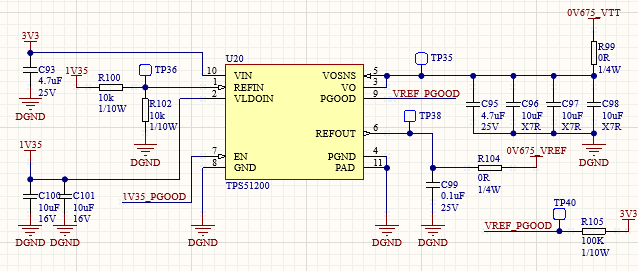
\includegraphics[scale=0.8]{images/refsupp.png}
    \caption{Regulador de tensão de referência e terminação para a memória DDR3L.}
    \label{fig:1v35ref}
    \fonte{Elaboração própria com base no circuito apresentado pelo fabricante.}
\end{figure}

\section{SoC}

No caso do SoC Zynq 7030, temos no total seis blocos operacionais, que incluem o funcionamento do PL e do PS, bem como as configurações e o bloco dedicado ao controlador da memória DDR (UG585, 2023). A seguir, estão dispostas as descrições funcionais e circuitos necessários para o funcionamento correto desse SoC, separados por cada um dos blocos citados.

\subsection{Bloco de Configuração}

O banco zero do SoC é o responsável por algumas opções e sinais de configuração. Abaixo, na Tabela \ref{tab:config}, se encontra a descrição funcional de cada pino desse banco, esquematizado na Figura \ref{fig:config}. Esse esquemático, bem como seus resistores de \textit{pull-up} (Figura \ref{fig:pullupconfig}), foram baseados na documentação técnica fornecida pela Xilinx (UG865, 2023) (UG470, 2023) (UG933, 2019) (DS191, 2018).


\begin{table}[H]
	\ABNTEXfontereduzida
	\caption{\label{tab:config}Descrição funcional dos pinos de configuração.}
	%\begin{tabular}{@{}p{2cm}p{2cm}p{2cm}p{2cm}p{2cm}p{2cm}p{3cm}@{}}
    \centering
    \begin{tabular}{@{} >{\centering}p{4cm} >{\centering}p{8cm} @{}}
    
		\toprule
		\textbf{Nome} & \textbf{Função} \tabularnewline 
        \midrule
         DXN e DXP & Terminais do diodo interno para medição de temperatura. \tabularnewline
         \midrule

         VREFP e VREFN & Tensões de referência do conversor analógico digital (XADC) do SoC. \tabularnewline

       \midrule
        VP e VN & Entrada extra do XADC. \tabularnewline

       \midrule
        VCCBAT & Não utilizada. Fonte da bateria. \tabularnewline

       \midrule
        TCK, TMS, TDI e TDO & Sinais da interface JTAG.  \tabularnewline

       \midrule
        INIT\_B & Indica inicialização da memória interna de configuração. \tabularnewline

       \midrule
       PROGRAM\_B & Reset assíncrono da lógica de configuração. \tabularnewline

       \midrule
        CFGBVS & Pino que seleciona o tipo de IO do banco 0. \tabularnewline

       \midrule
        DONE & Indica que a configuração foi terminada e feita corretamente. \tabularnewline

       \midrule
        VCCADC e GNDADC & Alimentação do XADC. \tabularnewline

       \midrule
        RSVDVCC e RSVDGND & Pinos de alimentação reservados. \tabularnewline

        \bottomrule
	\end{tabular}
	\fonte{Elaboração própria com base na documentação técnica do fabricante.}
\end{table}

\begin{figure}[H]
    \centering
    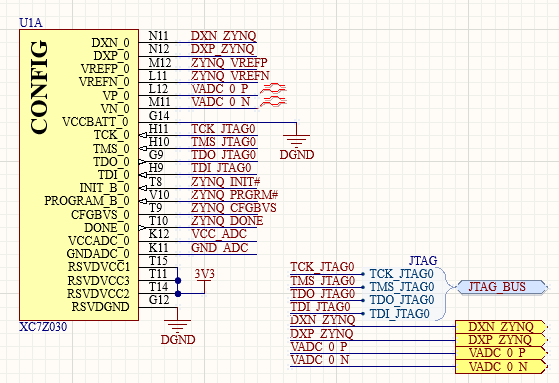
\includegraphics[scale=0.8]{images/zynqconfig.png}
    \caption{Banco de configuração do SoC.}
    \label{fig:config}
    \fonte{Elaboração própria com base no circuito apresentado pelo fabricante.}
\end{figure}

\begin{figure}[H]
    \centering
    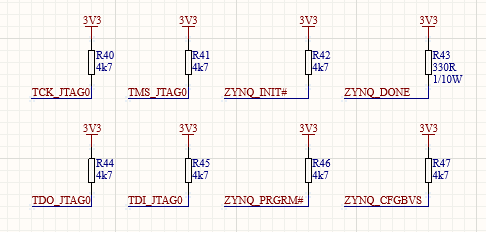
\includegraphics[scale=0.8]{images/pullupconfig.png}
    \caption{Resistores de \textit{pull-up} necessários.}
    \label{fig:pullupconfig}
    \fonte{Elaboração própria com base no circuito apresentado pelo fabricante.}
\end{figure}

Além disso, para a alimentação do XADC (\textit{Xilinx Analog to Digital Converter}), foi necessário um circuito de filtragem, disposto na Figura \ref{fig:xadcfilter}, como requerido por (UG480, 2022).

\begin{figure}[H]
    \centering
    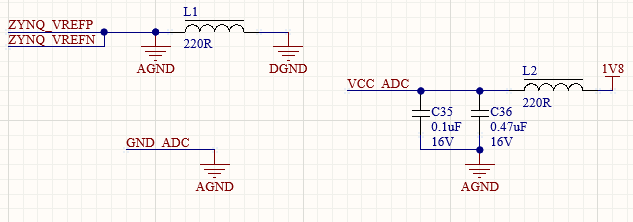
\includegraphics[scale=0.8]{images/xadcfilter.png}
    \caption{Filtro da alimentação analógica do SoC.}
    \label{fig:xadcfilter}
    \fonte{Elaboração própria com base no circuito apresentado pelo fabricante.}
\end{figure}


\subsection{Blocos do PS}

No caso do sistema de processamento (PS), existem três bancos principais. O primeiro, denominado MIO (\textit{Multiplexed In-Out}), é onde se encontram os controladores das interfaces de comunicação, bem como a entrada de relógio e a escolha do \textit{boot}. No caso desse projeto, foi-se decidido que o SoC poderá inicializar de duas formas, sendo a primeira pela interface JTAG e a segunda pela memória Flash NOR (QSPI), escolhidos pelos resistores R48 e R51. O banco MIO e seus modos de inicialização estão dispostos nas Figuras \ref{fig:psmio} e \ref{fig:boot}.

\begin{figure}[H]
    \centering
    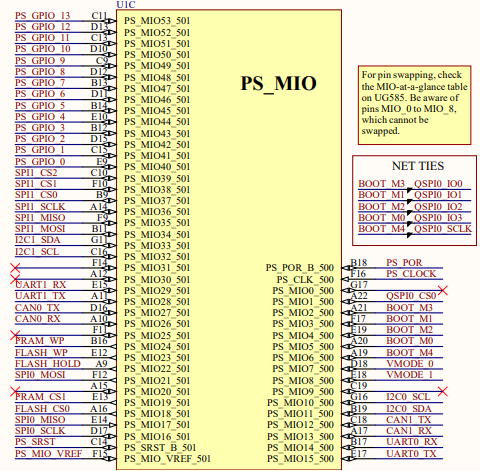
\includegraphics[scale=0.8]{images/psmio.png}
    \caption{Banco MIO do SoC com suas respectivas entradas e saídas.}
    \label{fig:psmio}
    \fonte{Elaboração própria com base na Tabela MIO-at-a-glance (UG585, 2023).}
\end{figure}

\begin{figure}[H]
    \centering
    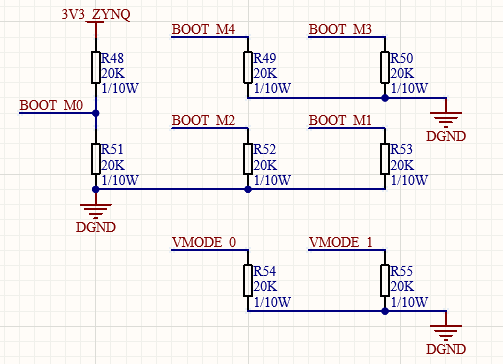
\includegraphics[scale=0.8]{images/bootmode.png}
    \caption{Modos de inicialização do SoC.}
    \label{fig:boot}
    \fonte{Elaboração própria com base em (UG585, 2023).}
\end{figure}

Por fim, Na Tabela \ref{tab:interfaces}, pode-se verificar qual a função de cada barramento de comunicação, em conformidade com a Figura \ref{fig:arq}. 

\begin{table}[H]
	\ABNTEXfontereduzida
	\caption{\label{tab:interfaces}Descrição das interfaces disponibilizadas.}
	%\begin{tabular}{@{}p{2cm}p{2cm}p{2cm}p{2cm}p{2cm}p{2cm}p{3cm}@{}}
    \centering
    \begin{tabular}{@{} >{\centering}p{4cm} >{\centering}p{8cm} @{}}
    
		\toprule
		\textbf{Interface} & \textbf{Função} \tabularnewline 
        \midrule
         SPI0 & Interface SPI para circuitos internos ao módulo OBDH. \tabularnewline
        \midrule
         SPI1 & Interface SPI para circuitos externos ao módulo OBDH.  \tabularnewline
        \midrule
         QSPI0 & Interface Quad-SPI para memória de inicialização. \tabularnewline
        \midrule
        I2C0  & Interface I2C para circuitos internos ao módulo OBDH. \tabularnewline
        \midrule
        I2C1  & Interface I2C para circuitos externos ao módulo OBDH.  \tabularnewline
        \midrule
        CAN0 & Interface CAN para circuitos externos ao módulo OBDH. \tabularnewline
        \midrule
        CAN1 & Interface CAN para o barramento de expansão. \tabularnewline
        \midrule
         UART0 & Conexão serial para \textit{debugging}. \tabularnewline
        \midrule
         UART1 & Conexão serial para o transceiver RS-485. \tabularnewline
        \midrule
         PS\_GPIO & Sinais de propósito geral de entrada e saída. \tabularnewline

        \bottomrule
	\end{tabular}
	\fonte{Elaboração própria com base na documentação técnica do fabricante.}
\end{table}

Também como mencionado, o projeto terá como memória volátil uma memória do tipo DDR3. Para que se consiga controlá-la, o SoC disponibiliza um banco dedicado para a memória DDR, disposto na  Figura \ref{fig:psddr}. Seus pinos são nomeados conforme (JEDEC, 2008) e suas funções são descritas na Tabela \ref{tab:psddr}. O terceiro banco não é utilizado nesse projeto.

\begin{figure}[H]
    \centering
    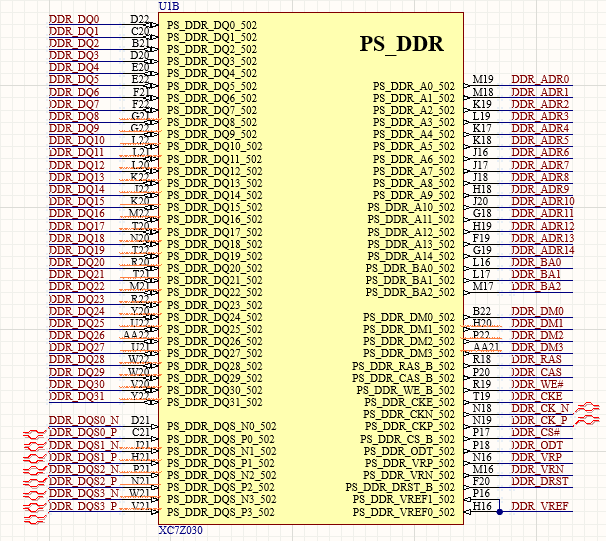
\includegraphics[scale=0.7]{images/psddr.png}
    \caption{Banco da Memória DDR do PS.}
    \label{fig:psddr}
    \fonte{Elaboração própria com base em (UG585, 2023) e (UG933, 2019).}
\end{figure}

\begin{table}[H]
	\ABNTEXfontereduzida
	\caption{\label{tab:psddr}Descrição dos pinos da memória DDR3.}
	%\begin{tabular}{@{}p{2cm}p{2cm}p{2cm}p{2cm}p{2cm}p{2cm}p{3cm}@{}}
    \centering
    \begin{tabular}{@{} >{\centering}p{4cm} >{\centering}p{8cm} @{}}
    
		\toprule
		\textbf{Nome} & \textbf{Descrição} \tabularnewline 
        \midrule
         DDR\_ADRx & Barramento de endereço da memória. \tabularnewline
        \midrule
         DDR\_DQx & Barramento de dados da memória. \tabularnewline
        \midrule
         DDR\_DMx & Sinal da máscara da interface. \tabularnewline
        \midrule
        DDR\_BAx  & Barramento de endereço do banco da memória. \tabularnewline
        \midrule
        DDR\_DQSx  & Sinal diferencial de \textit{Data Strobe}. \tabularnewline
        \midrule
        DDR\_CK & Barramento diferencial do relógio da memória. \tabularnewline
        \midrule
        DDR\_ODT & Sinal de saída de terminação dinâmica. \tabularnewline
        \midrule
        DDR\_CS\# & Sinal de \textit{Chip Select}. \tabularnewline
        \midrule
        DDR\_CKE & Sinal de \textit{enable} do relógio. \tabularnewline
        \midrule
        DDR\_WE\# & Sinal de \textit{Write Enable}. \tabularnewline
        \midrule
        DDR\_CAS & Sinal de endereço da coluna da memória. \tabularnewline
         \midrule
        DDR\_RAS & Sinal de endereço da linha da memória. \tabularnewline
        \midrule
        DDR\_DRST & Sinal de \textit{Reset}. \tabularnewline
        \bottomrule
	\end{tabular}
	\fonte{Elaboração própria com base em (UG585, 2023) e (JEDEC, 2008).}
\end{table}

\subsection{Blocos do PL}

O lado da FPGA do SoC, chamada de PL, é crucial para se ter um hardware versátil. Para isso, tentou-se utilizar a maior parte dos pinos possível, principalmente para o barramento externo. Nesses bancos também se encontram as entradas diferenciais do XADC do SoC. Nas Figuras \ref{fig:plhr} e \ref{fig:plhp} se encontram os esquemáticos dos bancos HR (\textit{High Range}) e HP (\textit{High Performance}), respectivamente. Na Tabela \ref{tab:plzynq}, por sua vez, se encontra a descrição funcional dos pinos por nome.

\begin{figure}[H]
    \centering
    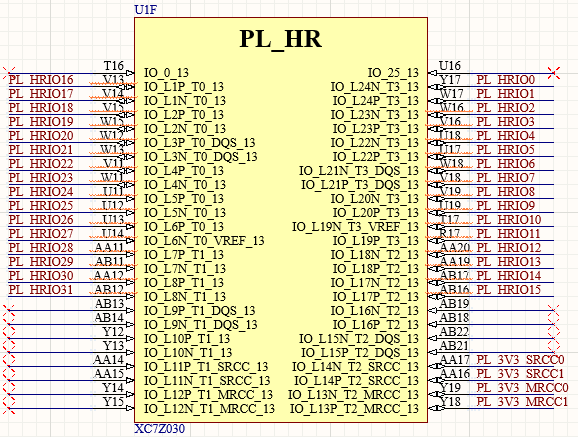
\includegraphics[scale=0.8]{images/plhr.png}
    \caption{Banco HR do PL.}
    \label{fig:plhr}
    \fonte{Elaboração própria com base em (UG585, 2023).}
\end{figure}

\begin{figure}[H]
    \centering
    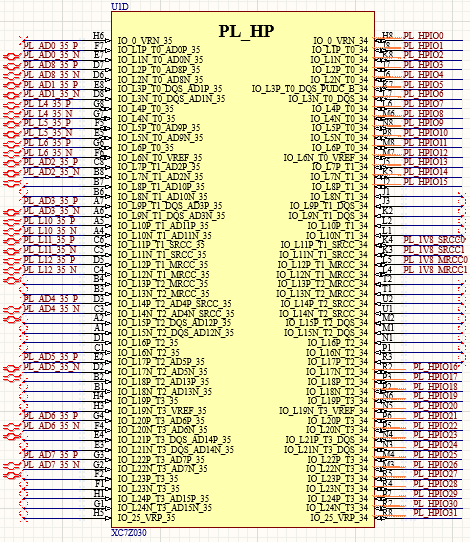
\includegraphics[scale=0.7]{images/plhp.png}
    \caption{Banco HP do PL.}
    \label{fig:plhp}
    \fonte{Elaboração própria com base em (UG585, 2023).}
\end{figure}

\begin{table}[H]
	\ABNTEXfontereduzida
	\caption{\label{tab:plzynq}Descrição dos sinais dos bancos do PL.}
	%\begin{tabular}{@{}p{2cm}p{2cm}p{2cm}p{2cm}p{2cm}p{2cm}p{3cm}@{}}
    \centering
    \begin{tabular}{@{} >{\centering}p{4cm} >{\centering}p{8cm} @{}}
    
		\toprule
		\textbf{Nome} & \textbf{Descrição} \tabularnewline 
        \midrule
         PL\_ADx & Entrada diferencial enumerada do XADC. \tabularnewline
        \midrule
         PL\_Lx & Sinal LVDS, presente apenas no banco HP. \tabularnewline
        \midrule
         PL\_HPIOx & Sinal de entrada e saída genérico do banco HP.  \tabularnewline
        \midrule
        PL\_HRIOx  & Sinal de entrada e saída genérico do banco HR. \tabularnewline
        \midrule
        PL\_xx\_SRCCx & Pino capaz de gerar sinal de relógio do tipo \textit{Single Region}. \tabularnewline
        \midrule
        PL\_xx\_MRCCx & Pino capaz de gerar sinal de relógio do tipo \textit{Multi Region}. \tabularnewline
        \bottomrule
	\end{tabular}
	\fonte{Elaboração própria com base em (UG585, 2023).}
\end{table}

\subsection{Pinos de Potência}

Por fim, os pinos de potência devem ser alimentados corretamente. Além disso, é recomendado por (UG933, 2019) que todos os pinos tenham capacitores de desacoplamento o mais perto possível de seus respectivos pinos. Esse circuito e seus capacitores estão dispostos nas Figuras \ref{fig:zpower} e \ref{fig:zcaps}.

\begin{figure}[H]
    \centering
    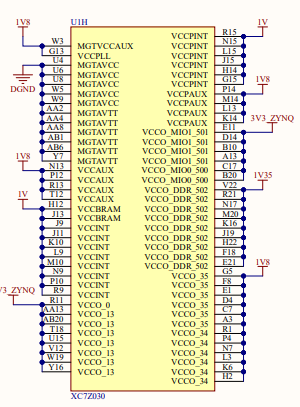
\includegraphics[scale=0.7]{images/zynqpower.png}
    \caption{Pinos de potência do SoC.}
    \label{fig:zpower}
    \fonte{Elaboração própria com base em (UG585, 2023) e (UG933, 2019).}
\end{figure}

\begin{figure}[H]
    \centering
    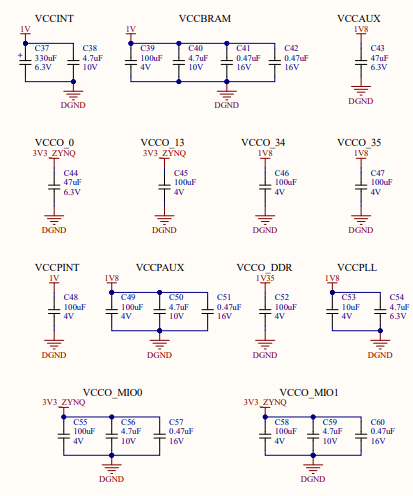
\includegraphics[scale=0.7]{images/zynqcaps.png}
    \caption{Capacitores de desacoplamento recomendados.}
    \label{fig:zcaps}
    \fonte{(UG933, 2019).}
\end{figure}

\section{Memórias}

Nesta seção, abordam-se as principais características das memórias utilizadas no sistema. Serão comentados os circuitos das memórias DDR3L, das memórias Flash NAND e NOR e da memória FRAM.

\subsection{DDR3L} 

A DDR3L selecionada oferece 2 Gb de capacidade de armazenamento, configurada em uma estrutura de 256M x 8 bits. Essa memória opera com tensão reduzida (1.35V), o que a torna eficiente em termos de consumo de energia, crucial para sistemas de satélite. Seu circuito se encontra na Figura \ref{fig:ddr3l}. 

\begin{figure}[H]
    \centering
    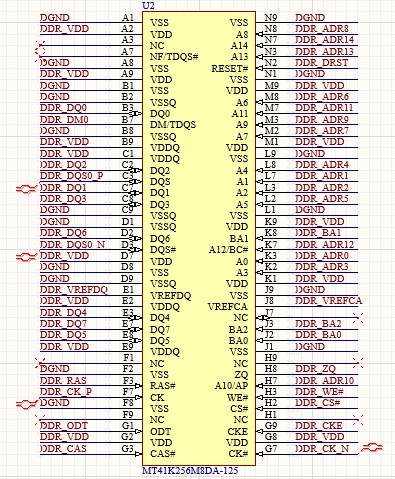
\includegraphics[scale=0.7]{images/ddr3l.png}
    \caption{Circuito da memória DDR3L.}
    \label{fig:ddr3l}
    \fonte{(MT41K256M8DA-125:K DDR3L Datasheet).}
\end{figure}

\subsection{Flash NOR}

A memória flash NOR, acessada por uma interface QSPI, foi escolhida pela sua capacidade de realizar leituras rápidas, característica que torna esse tipo de memória adequado para armazenamento de firmware ou dados de inicialização do sistema. Seu circuito está presente na Figura \ref{fig:fnor}.

\begin{figure}[H]
    \centering
    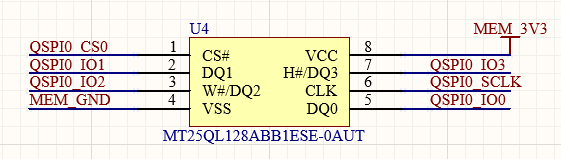
\includegraphics[scale=0.7]{images/flash nor.png}
    \caption{Circuito da memória Flash NOR.}
    \label{fig:fnor}
    \fonte{(MT25QL128ABB1ESE-0AUT Flash NOR Datasheet).}
\end{figure}

\subsection{Flash NAND}

Diferente da flash NOR, a memória flash NAND, acessada via SPI, é utilizada para armazenamento de grandes volumes de dados que não necessitam de acesso frequente, ou seja, dados de uso prolongado, como logs e registros. Seu circuito se encontra na Figura \ref{fig:fnand}.

\begin{figure}[H]
    \centering
    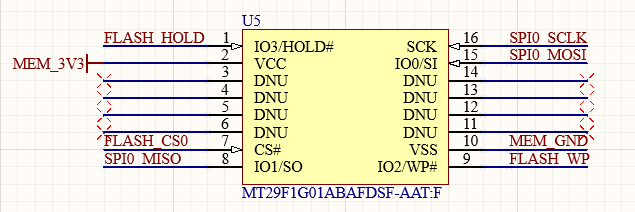
\includegraphics[scale=0.7]{images/flash nand.png}
    \caption{Circuito da memória Flash NAND.}
    \label{fig:fnand}
    \fonte{(MT29F1G01ABAFDSF-AAT:F Flash NAND Datasheet).}
\end{figure}

\subsection{FRAM}

 A FRAM, com acesso por interface SPI, será usada para armazenar dados críticos por sua alta resistência a radiação e alta velocidade de escrita e leitura. Seu circuito se encontra na Figura \ref{fig:fram}.

\begin{figure}[H]
    \centering
    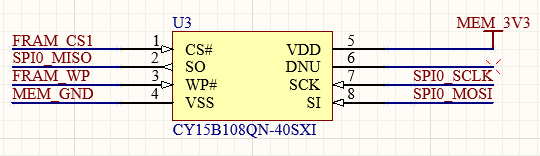
\includegraphics[scale=0.7]{images/fram.png}
    \caption{Circuito da memória FRAM.}
    \label{fig:fram}
    \fonte{(CY15B104QN FRAM Datasheet).}
\end{figure}

\section{Periféricos}

Como previsto nos requisitos, são necessários os circuitos do WDT, dos sensores de tensão, corrente e temperatura e do sistema do ADCS. 

Primeiramente, o circuito do WDT, disposto na Figura \ref{fig:wdt}, foi construído para reinicializar o SoC caso o sinal de controle (WDI) não mude por mais de 1,6 segundos (tipicamente). Além disso, o circuito integrado é equipado com um sinal de \textit{reset} manual. 

\begin{figure}[H]
    \centering
    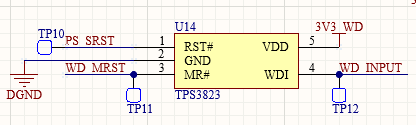
\includegraphics[scale=0.7]{images/wdt.png}
    \caption{Circuito do WDT.}
    \label{fig:wdt}
    \fonte{(TPS3823-33QDBVRQ1 Watchdog Timer Datasheet).}
\end{figure}

No circuito do sensor de tensão e temperatura, são monitoradas as tensões de 1 V, 1,8 V, 1,35 V e  0,675 V. Além disso, são medidas as temperaturas tanto do SoC, através dos sinais DXP e DXN, provenientes do diodo interno do Zynq (UG865, 2021), quanto a temperatura da placa, em um transistor externo. O mesmo está disposto na Figura \ref{fig:sense}.

\begin{figure}[H]
    \centering
    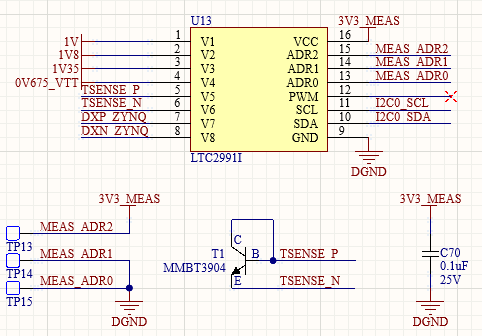
\includegraphics[scale=0.7]{images/sense.png}
    \caption{Circuito do monitor de tensão e temperatura.}
    \label{fig:sense}
    \fonte{(LTC2991IMS\#TRPBF Voltage, Current and Temperature Monitor Datasheet).}
\end{figure}

Quanto ao circuito de medição de corrente, foi necessário o cálculo do resistor de medição (Rsense), presente em (6) (INA180A2IDBVR Current Sense Datasheet). Com o valor máximo de Rsense, foi escolhido um resistor menor, de 75 m$\Omega$, para obter uma margem com relação à corrente máxima. Sua saída é lida por uma entrada do XADC do SoC. Seu circuito final está disposto na Figura \ref{fig:csense}.

\begin{equation}
	R_{sense} < Vsp / (G \times Imax) = 1 / (50 \times 2,5) = 80 m\Omega
\end{equation} 

\begin{figure}[H]
    \centering
    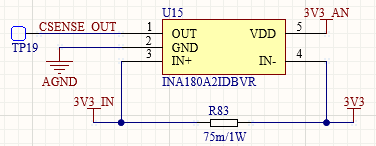
\includegraphics[scale=0.7]{images/current sense.png}
    \caption{Circuito de medição de corrente.}
    \label{fig:csense}
    \fonte{(INA180A2IDBVR Current Sense Datasheet).}
\end{figure}

Por fim, o sistema ADCS, controlado pela interface I2C0, será formado pelos circuitos das Figuras \ref{fig:mag} e \ref{fig:gyro}, do magnetômetro e do giroscópio. 

\begin{figure}[H]
    \centering
    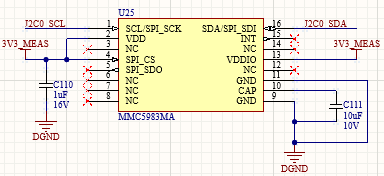
\includegraphics[scale=0.7]{images/magnetometer.png}
    \caption{Circuito do magnetômetro.}
    \label{fig:mag}
    \fonte{(MMC5983MA Magnetometer Datasheet).}
\end{figure}

\begin{figure}[H]
    \centering
    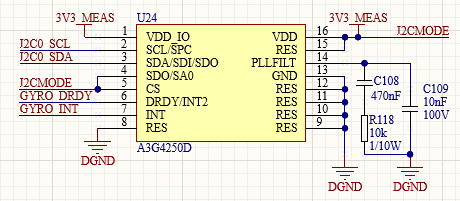
\includegraphics[scale=0.7]{images/gyro.png}
    \caption{Circuito do giroscópio.}
    \label{fig:gyro}
    \fonte{(A3G4250D Gyroscope Datasheet).}
\end{figure}

\section{Conexões entre blocos}

Por fim, todos os blocos foram conectados, usando o princípio de projeto hierárquico fornecido pelo \textit{software} utilizado. A interconexão leva em conta a arquitetura proposta e as necessidades individuais de cada subcircuito apresentado no presente capítulo. Seu esquemático está disposto na Figura \ref{fig:inter}.

\begin{figure}[H]
    \centering
    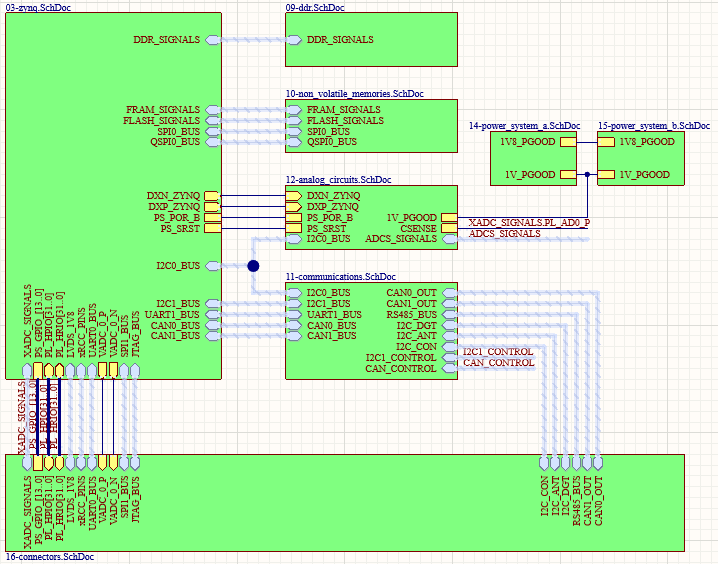
\includegraphics[scale=0.7]{images/conexoes.png}
    \caption{Interconexão dos blocos propostos.}
    \label{fig:inter}
    \fonte{Elaboração própria.}
\end{figure}

% ----------------------------------------------------------
\chapter{Resultados}
% ----------------------------------------------------------
% ----------------------------------------------------------
\chapter{Considerações finais}
% ----------------------------------------------------------
O desenvolvimento deste trabalho teve como principal objetivo a criação de uma arquitetura de hardware robusta e versátil para um computador de bordo destinado a pequenos satélites, especificamente CubeSats. Este computador de bordo foi projetado para operar em ambientes espaciais adversos, assegurando a integridade e a confiabilidade no tratamento de dados, além de possibilitar a adaptação a diferentes tipos de missões e experimentos científicos em órbita.

Dentre os objetivos específicos, estavam a análise dos requisitos de robustez para ambientes espaciais, a especificação de uma arquitetura adaptável e a documentação detalhada de todas as decisões de projeto. Para atender esses objetivos, inicialmente, a robustez do sistema foi trabalhada com a seleção cuidadosa de componentes eletrônicos que pudessem resistir a fatores ambientais como radiação e temperatura extrema, presentes em LEO. Tais componentes foram escolhidos de acordo com diretrizes de herança de voo e normas estabelecidas pela ESA e NASA, de forma a garantir maior confiabilidade e segurança operacional.

No aspecto da versatilidade, o sistema foi arquitetado de modo a integrar memórias, sensores e periféricos variados, de modo a atender a diferentes tipos de missões. Esse objetivo foi cumprido por meio do uso de um SoC da família Zynq, que incorpora um microprocessador e uma FPGA, conferindo ao sistema uma alta adaptabilidade. As interfaces genéricas disponibilizadas para os conectores (SPI, I2C, UART, CAN e diversos pinos de entrada e saída genéricos), também corroboraram para essa versatilidade, permitindo a interconexão com muitos componentes diferentes.

Outro aspecto relevante abordado neste projeto foi a robustez das interfaces de comunicação. Para garantir a integridade das transmissões de dados entre os módulos do CubeSat, optou-se pela utilização da interface CAN, que oferece maior resistência a interferências, sendo especialmente adequadas para sistemas embarcados que exigem alta confiabilidade. Além disso, o sistema conta com sensores para monitoramento de temperatura, tensão e corrente, componentes essenciais para a operação segura e para a prevenção de falhas.

A abordagem de modularidade do projeto também reforça sua robustez e flexibilidade. Com o uso de memórias não voláteis (Flash NOR, Flash NAND e FRAM) para o armazenamento de dados críticos e a inicialização segura do sistema, o computador de bordo projetado consegue resistir às adversidades do ambiente espacial. Além disso, cada componente foi avaliado quanto ao consumo energético e às exigências de funcionamento entre -40°C e 85 °C.

Conclui-se que o projeto realizado cumpre os objetivos propostos, apresentando uma solução robusta, segura e adaptável para a operação em CubeSats. A flexibilidade conferida pela arquitetura de SoC com FPGA integrada, associada à robustez das interfaces e ao uso de memórias especializadas, permite que o sistema seja facilmente adaptável a diferentes \textit{payloads}. Dessa forma, esse trabalho contribui para o avanço das tecnologias embarcadas em pequenos satélites, oferecendo uma base confiável e versátil para futuras inovações em missões espaciais.







\begin{flushleft}
\begin{thebibliography}{00} %59
\bibitem{b1} AAC Clyde Space. \textbf{Datasheet: Kryten-M3}. Disponível em $<$https://www.aac-clyde.space/wp-content/uploads/2021/10/AAC\_DataSheet\_Kryten.pdf$>$.  Acesso em: 07 jun. 2024.

\bibitem{b36} \textbf{A3G4250D Gyroscope Datasheet}. Disponível em: $<$\url{https://www.st.com/content/ccc/resource/technical/document/datasheet/5c/f1/a4/70/1b/fa/40/d2/DM00047823.pdf/files/DM00047823.pdf/jcr:content/translations/en.DM00047823.pdf}$>$. Acesso em: 27 out. 2024. 

\bibitem{b21} \textbf{AN-600: Understanding Latch-Up in Advanced CMOS Logic}. [s.l: s.n.]. Disponível em: $<$https://large.stanford.edu/courses/2015/ph241/clark2/docs/AN-600.pdf$>$. Acesso em: 26 out. 2024.

\bibitem{b48} BARLES, A. et al. \textbf{Mission ORCA: Orbit refinement for collision avoidance}. Advances in Astronautics Science and Technology, v. 5, n. 2, p. 149–165, 2022.

%\bibitem{b57} BOING, M. \textbf{Técnicas de mitigação de efeitos da radiação e sua aplicação no projeto de uma arquitetura de hardware para uso em satélites}. Florianópolis, SC: UFSC, 19 de julho de 2024.

\bibitem{b56} BOUKHOBZA, J.; OLIVIER, P. \textbf{Emerging Non-volatile Memories}. Em: Flash Memory Integration. [s.l.] Elsevier, 2017. p. 203–224.

\bibitem{b40} CADENCE PCB SOLUTIONS. \textbf{Zener diode applications: Circuit protection}. Disponível em: <https://resources.pcb.cadence.com/blog/2023-zener-diode-applications-circuit-protection>. Acesso em: 28 out. 2024

\bibitem{b13} CARMO, T. A.; MOREIRA , J. Q.; MANEA, S. \textbf{Análise de blindagem à radiação “TID” e “SEU” em memória do tipo SRAM em orbita LEO (Low Earth Orbit)}. 12° Workshop em Engenharia e Tecnologia Espaciais, 6 nov. 2021.

\bibitem{b49} CAMPS, A. et al. \textbf{Fsscat, the 2017 Copernicus masters’ “Esa sentinel small satellite challenge” winner: A federated polar and soil moisture tandem mission based on 6U cubesats}. IGARSS 2018 - 2018 IEEE International Geoscience and Remote Sensing Symposium. Anais...IEEE, 2018.

\bibitem{b2} CAPPELLETTI, C.; BATTISTINI, S.; MALPHRUS, B. \textbf{Cubesat Handbook: From Mission Design to Operations}. Editora Elsevier, 2021.

\bibitem{b58} \textit{CubeSat101: Basic Concepts and Processes for First-Time CubeSat Developers}. [S.l.: s.n.], 2017. Disponível em $<$https://www.nasa.gov/wp-content/uploads/2017/03/nasa\_csli\_cubesat\_101\_508.pdf?emrc=05d3e2$>$. Acesso em 28 out. 2024.

\bibitem{b15} \textbf{CUBESAT Design Specification}. [S.l.: s.n.], 2022. Disponível em $<$https://www.cubesat.org/cubesatinfo$>$. Acesso em: 25 out. 2024.

\bibitem{b22} \textbf{CY15B104QN FRAM Datasheet}. Disponível em: $<$\url{https://www.infineon.com/dgdl/Infineon-CY15B104QN\_CY15V104QN\_Excelon(TM)\_LP\_4-Mbit\_(512K\_X\_8)\_Serial\_(SPI)\_F-RAM-DataSheet-v12\_00-EN.pdf?fileId=8ac78c8c7d0d8da4017d0ee7709b704a\&utm\_source=cypress\&utm\_medium=referral\&utm\_campaign=202110\_globe\_en\_all\_integr}$>$. Acesso em: 27 out. 2024.

\bibitem{b47} \textbf{DS191 - Zynq-7000 SoC (Z-7030, Z-7035, Z-7045, and Z-7100): DC and AC Switching Characteristics}. 2018. Disponível em $<$https://docs.amd.com/v/u/en-US/ds191-XC7Z030-XC7Z045-data-sheet$>$. Acesso em: 29 out. 2024.

\bibitem{b14} ECSS. \textbf{ECSS-Q-ST-60C Rev.3 – Electrical, electronic and electromechanical (EEE) components (12 May 2022)}. Disponível em: $<$https://ecss.nl/standard/ecss-q-st-60c-rev-3-electrical-electronic-and-electromechanical-eee-components-2-may-2022/$>$. Acesso em: 6 out. 2024.

\bibitem{b57} ECSS. \textbf{ECSS-E-ST-10-04C - Space Environment}. The Netherlands: [s.n.], 2008.

\bibitem{b20} GERARDIN, S.; PACCAGNELLA, A. \textbf{Present and future non-volatile memories for space}. IEEE transactions on nuclear science, 2010.

\bibitem{b3} GEORGE, A. D.; WILSON, C. M. \textbf{Onboard processing with hybrid and reconfigurable computing on small satellites}. Proceedings of the IEEE. Institute of Electrical and Electronics Engineers, 2018.

\bibitem{b4} \textbf{Gomspace NanoMind A3200 Datasheet}. Disponível em $<$https://gomspace.com/UserFiles/Subsystems/datasheet/gs-ds-nanomind-a3200\_1006901-117.pdf$>$. Acesso em: 07 jun. 2024.

\bibitem{b5} \textbf{Gomspace NanoMind HP MK3 Datasheet}. Disponível em $<$https://gomspace.com/UserFiles/Subsystems/datasheet/gs-ds-NanoMind\_HP\_MK3.pdf$>$. Acesso em: 07 jun. 2024.

\bibitem{b51} \textbf{Gomspace Nanomind Z7000 Datasheet}. 2019. Disponível em: $<$https://gomspace.com/UserFiles/Subsystems/datasheet/gs-ds-nanomind-z7000-15.pdf$>$. Acesso em: 30 oct. 2024.

\bibitem{b34} \textbf{INA180A2IDBVR Current Sense Datasheet}. Disponível em: $<$\url{https://www.ti.com/lit/ds/symlink/ina180.pdf?HQS=dis-dk-null-digikeymode-dsf-pf-null-wwe\&ts=1727202734954\&ref\_url=https\%253A\%252F\%252Fwww.ti.com\%252Fgeneral\%252Fdocs\%252Fsuppproductinfo.tsp\%253FdistId\%253D10\%2526gotoUrl\%253Dhttps\%253A\%252F\%252Fwww.ti.com\%252Flit\%252Fgpn\%252Fina180}$>$. Acesso em: 27 out. 2024. 

\bibitem{b6} \textbf{ISIS Space On Board Computer}. Disponível em $<$https://www.isispace.nl/product/on-board-computer/$>$. Acesso em: 07 jun. 2024.

\bibitem{b19} JEDEC. \textbf{Double Data Rate (DDR) SDRAM Standard}. 2008. Disponível em: $<$https://www.jedec.org/standards-documents/docs/jesd-79f$>$. Acesso em: 26 out. 2024.

\bibitem{b10} JUNQUEIRA, B. C.; MANEA, S.\textbf{Utilização de COTS em nano satélites}. Brazilian Journal of Development, v. 6, n. 1, p. 1476-1490, 2020.

\bibitem{b16} KADI, M. A. et al. \textbf{Dynamic and partial reconfiguration of Zynq 7000 under Linux}. 2013 International Conference on Reconfigurable Computing and FPGAs (ReConFig). Anais...IEEE, 2013.

\bibitem{b18} KLEHN, B.; BROX, M. A. \textbf{Comparison of current SDRAM types: SDR, DDR, and RDRAM}. Advances in radio science, v. 1, p. 265–271, 2003.

\bibitem{b59} LABEL, K. A. \textbf{Radiation Effects on Electronics 101: Simple Concepts and New Challenges}. NEPP Webex Presentation, 2004.

\bibitem{b54} LOFFLER, T. et al. \textbf{Research and Observation in Medium Earth Orbit (ROMEO) with a cost-effective microsatellite platform}. 72nd International Astronautical Congress (IAC), Dubai, United Arab Emirates. 2021. 

\bibitem{b12} \textbf{Low earth orbit}. Disponível em: $<$https://www.esa.int/ESA\_Multimedia/Images/2020/03/Low\_Earth\_orbit$>$. Acesso em: 6 out. 2024.

\bibitem{b27} \textbf{LTC2991IMS\#TRPBF Voltage, Current and Temperature Monitor Datasheet}. Disponível em: $<$https://www.analog.com/media/en/technical-documentation/data-sheets/2991ff.pdf$>$. Acesso em: 27 out. 2024. 

\bibitem{b37} \textbf{LTC4361 Overcurrent Protection Controller Datasheet}. 2018. Disponível em: $<$https://www.analog.com/media/en/technical-documentation/data-sheets/LTC4361-1-4361-2.pdf$>$. Acesso em: 27 out. 2024. 

\bibitem{b11} MAYANBARI, Masood; KASESAZ, Yaser. \textbf{Design and analyse space radiation shielding for a nanosatellite in Low Earth Orbit (LEO)}. In: Proceedings of 5th International Conference on Recent Advances in Space Technologies-RAST2011. IEEE, 2011. p. 489-493.

\bibitem{b42} MAK, B. \textbf{Basics of Load Switches}. 2018. Disponível em: <https://www.ti.com/lit/an/slva652a/slva652a.pdf?ts=1730079105016>. Acesso em: 28 out. 2024.

\bibitem{b8} MARCELINO, G. M. et al. \textbf{A critical embedded system challenge: The FloripaSat-1 mission}. IEEE Latin America Transactions, 2020.

\bibitem{b9} MARCELINO, G. M. et al. \textbf{FloripaSat-2: An Open-Source Platform for CubeSats}. IEEE embedded systems letters, 2024.

\bibitem{b35} \textbf{MMC5983MA Magnetometer Datasheet}. Disponível em: $<$\url{https://mm.digikey.com/Volume0/opasdata/d220001/medias/docus/333/MMC5983MA\_RevA\_4-3-19.pdf}$>$. Acesso em: 27 out. 2024. 

\bibitem{b25} \textbf{MT25QL128ABB1ESE-0AUT Flash NOR Datasheet}. Disponível em: $<$https://www.micron.com/content/dam/micron/global/secure/products/data-sheet/nor-flash/serial-nor/mt25q/die-rev-b/mt25q-qlht-l-128-abb-xxt.pdf$>$. Acesso em: 27 out. 2024. 

\bibitem{b24} \textbf{MT29F1G01ABAFDSF-AAT:F Flash NAND Datasheet}. Disponível em: $<$https://www.micron.com/content/dam/micron/global/secure/products/data-sheet/nand-flash/70-series/m78a-1gb-spi-auto.pdf$>$. Acesso em: 27 out. 2024. 

\bibitem{b23} \textbf{MT41K256M8DA-125:K DDR3L Datasheet}. Disponível em: $<$https://www.micron.com/content/dam/micron/global/secure/products/data-sheet/dram/ddr3/2gb-1-35v-ddr3l.pdf$>$. Acesso em: 27 out. 2024. 

\bibitem{b7} Nano Avionics. \textbf{CubeSat On-Board Computer – Main Bus Unit SatBus 3C2}. Disponível em $<$https://nanoavionics.com/cubesat-components/cubesat-on-board-computer-main-bus-unit-satbus-3c2/$>$. Acesso em: 07 jun. 2024.

\bibitem{b13} \textbf{NASA Parts Selection List (NPSL)}. Disponível em: $<$https://nepp.nasa.gov/npsl/$>$. Acesso em: 6 out. 2024.

\bibitem{b55} \textbf{NASA Product Verification}. Disponível em: $<$https://www.nasa.gov/reference/5-3-product-verification/$>$. Acesso em: 30 out. 2024.

\bibitem{b53} PUTRA, A. C. A. Y.; WIJANTO, H.; EDWAR. \textbf{Design and implementation RTOS (real time operating system) as a nano satellite control for responding to space environmental conditions}. 2021 IEEE Asia Pacific Conference on Wireless and Mobile (APWiMob). Anais...IEEE, 2021.

\bibitem{b41} SARJEANT, W. \textbf{Capacitors}. IEEE transactions on electrical insulation, v. 25, n. 5, p. 861–922, 1990.

\bibitem{b39} SOH, W.-S. et al. \textbf{Filter design for suppression of noise coupling from PCB to DC power supply}. 2010 Asia-Pacific International Symposium on Electromagnetic Compatibility. Anais...IEEE, 2010.

\bibitem{b28} \textbf{TCA4311ADR I2C Buffer Datasheet}. Disponível em: $<$\url{https://www.ti.com/general/docs/suppproductinfo.tsp?distId=10\&gotoUrl=https\%3A\%2F\%2Fwww.ti.com\%2Flit\%2Fgpn\%2Ftca4311a}$>$. Acesso em: 27 out. 2024. 

\bibitem{b33} \textbf{TCAN330D CAN Transceiver Datasheet}. Disponível em: $<$\url{https://www.ti.com/lit/ds/symlink/tcan330.pdf?ts=1729084231140\&ref\_url=https\%253A\%252F\%252Fbr.mouser.com\%252F}$>$. Acesso em: 27 out. 2024. 

\bibitem{b29} \textbf{THVD1451DR RS-485 Transceiver Datasheet}. Disponível em: $<$\url{https://www.ti.com/lit/ds/symlink/thvd1410.pdf?HQS=dis-dk-null-digikeymode-dsf-pf-null-wwe\&ts=1722094226249\&ref\_url=https\%253A\%252F\%252Fwww.ti.com\%252Fgeneral\%252Fdocs\%252Fsuppproductinfo.tsp\%253FdistId\%253D10\%2526gotoUrl\%253Dhttps\%253A\%252F\%252Fwww.ti.com\%252Flit\%252Fgpn\%252Fthvd1410}$>$. Acesso em: 27 out. 2024. 

\bibitem{b30} \textbf{TPS22920YZPR Load Switch Datasheet}. 2016. Disponível em: $<$\url{https://www.ti.com/general/docs/suppproductinfo.tsp?distId=10\&gotoUrl=https\%3A\%2F\%2Fwww.ti.com\%2Flit\%2Fgpn\%2Ftps22920}$>$. Acesso em: 27 out. 2024. 

\bibitem{b26} \textbf{TPS3823-33QDBVRQ1 Watchdog Timer Datasheet}. Disponível em: $<$\url{https://www.ti.com/general/docs/suppproductinfo.tsp?distId=10\&gotoUrl=https\%3A\%2F\%2Fwww.ti.com\%2Flit\%2Fgpn\%2Ftps3828-q1}$>$. Acesso em: 27 out. 2024. 

\bibitem{b31} \textbf{TPS51200DRCR DC-DC Voltage Regulator Datasheet}. Disponível em: $<$\url{https://www.ti.com/general/docs/suppproductinfo.tsp?distId=10\&gotoUrl=https\%3A\%2F\%2Fwww.ti.com\%2Flit\%2Fgpn\%2Ftps51200}$>$. Acesso em: 27 out. 2024. 

\bibitem{b32} \textbf{TPS82085SILR DC-DC Voltage Regulator Datasheet}. 2019. Disponível em: $<$\url{https://www.ti.com/general/docs/suppproductinfo.tsp?distId=10\&gotoUrl=https\%3A\%2F\%2Fwww.ti.com\%2Flit\%2Fgpn\%2Ftps82085}$>$. Acesso em: 27 out. 2024. 

\bibitem{b44} \textbf{UG470 - 7 Series FPGAs Configuration User Guide}. 2023. Disponível em $<$https://docs.amd.com/v/u/en-US/ug470\_7Series\_Config$>$. Acesso em: 29 out. 2024.

\bibitem{b45} \textbf{UG480 - 7 Series FPGAs and Zynq-7000 SoC XADC Dual 12-Bit 1 MSPS Analog-to-Digital Converter User Guide}. 2022. Disponível em $<$https://docs.amd.com/r/en-US/ug480\_7Series\_XADC$>$. Acesso em: 29 out. 2024.

\bibitem{b38} \textbf{UG585 - Zynq 7000 SoC Technical Reference Manual - AMD technical information portal}. 2023. Disponível em: $<$https://docs.amd.com/r/en-US/ug585-zynq-7000-SoC-TRM/Zynq-7000-SoC-Technical-Reference-Manual$>$. Acesso em: 25 out. 2024.

\bibitem{b17} \textbf{UG865 - Zynq-7000 SoC Packaging and Pinout Product Specification - AMD technical information portal}. 2021. Disponível em: $<$https://docs.amd.com/v/u/en-US/ug865-Zynq-7000-Pkg-Pinout$>$. Acesso em: 25 out. 2024.

\bibitem{b46} \textbf{UG933 - Zynq-7000 SoC PCB Design Guide}. 2019. Disponível em $<$https://docs.amd.com/v/u/en-US/ug933-Zynq-7000-PCB$>$. Acesso em: 29 out. 2024.

\bibitem{b50} WEIDMANN, D. et al. \textbf{Cubesats for monitoring atmospheric processes (CubeMAP): a constellation mission to study the middle atmosphere}. Sensors, Systems, and Next-Generation Satellites XXIV. Anais...SPIE, 2020.

\bibitem{b43} \textbf{XPE - Power Estimator}. 2019. Disponível em: $<$https://www.amd.com/en/products/adaptive-socs-and-fpgas/technologies/power-efficiency/power-estimator.html$>$. Acesso em: 28 out. 2024.

\bibitem{b52} ZHOU, Q. et al. \textbf{Design of a compact and reconfigurable onboard data handling system}. 2018 IEEE Intl Conf on Parallel \& Distributed Processing with Applications, Ubiquitous Computing \& Communications, Big Data \& Cloud Computing, Social Computing \& Networking, Sustainable Computing \& Communications (ISPA/IUCC/BDCloud/SocialCom/SustainCom). Anais...IEEE, 2018.

\end{thebibliography}
\end{flushleft}


\postextual
%\begin{flushleft}
\begin{thebibliography}{00} %59
\bibitem{b1} AAC Clyde Space. \textbf{Datasheet: Kryten-M3}. Disponível em $<$https://www.aac-clyde.space/wp-content/uploads/2021/10/AAC\_DataSheet\_Kryten.pdf$>$.  Acesso em: 07 jun. 2024.

\bibitem{b36} \textbf{A3G4250D Gyroscope Datasheet}. Disponível em: $<$\url{https://www.st.com/content/ccc/resource/technical/document/datasheet/5c/f1/a4/70/1b/fa/40/d2/DM00047823.pdf/files/DM00047823.pdf/jcr:content/translations/en.DM00047823.pdf}$>$. Acesso em: 27 out. 2024. 

\bibitem{b21} \textbf{AN-600: Understanding Latch-Up in Advanced CMOS Logic}. [s.l: s.n.]. Disponível em: $<$https://large.stanford.edu/courses/2015/ph241/clark2/docs/AN-600.pdf$>$. Acesso em: 26 out. 2024.

\bibitem{b48} BARLES, A. et al. \textbf{Mission ORCA: Orbit refinement for collision avoidance}. Advances in Astronautics Science and Technology, v. 5, n. 2, p. 149–165, 2022.

%\bibitem{b57} BOING, M. \textbf{Técnicas de mitigação de efeitos da radiação e sua aplicação no projeto de uma arquitetura de hardware para uso em satélites}. Florianópolis, SC: UFSC, 19 de julho de 2024.

\bibitem{b56} BOUKHOBZA, J.; OLIVIER, P. \textbf{Emerging Non-volatile Memories}. Em: Flash Memory Integration. [s.l.] Elsevier, 2017. p. 203–224.

\bibitem{b40} CADENCE PCB SOLUTIONS. \textbf{Zener diode applications: Circuit protection}. Disponível em: <https://resources.pcb.cadence.com/blog/2023-zener-diode-applications-circuit-protection>. Acesso em: 28 out. 2024

\bibitem{b13} CARMO, T. A.; MOREIRA , J. Q.; MANEA, S. \textbf{Análise de blindagem à radiação “TID” e “SEU” em memória do tipo SRAM em orbita LEO (Low Earth Orbit)}. 12° Workshop em Engenharia e Tecnologia Espaciais, 6 nov. 2021.

\bibitem{b49} CAMPS, A. et al. \textbf{Fsscat, the 2017 Copernicus masters’ “Esa sentinel small satellite challenge” winner: A federated polar and soil moisture tandem mission based on 6U cubesats}. IGARSS 2018 - 2018 IEEE International Geoscience and Remote Sensing Symposium. Anais...IEEE, 2018.

\bibitem{b2} CAPPELLETTI, C.; BATTISTINI, S.; MALPHRUS, B. \textbf{Cubesat Handbook: From Mission Design to Operations}. Editora Elsevier, 2021.

\bibitem{b58} \textit{CubeSat101: Basic Concepts and Processes for First-Time CubeSat Developers}. [S.l.: s.n.], 2017. Disponível em $<$https://www.nasa.gov/wp-content/uploads/2017/03/nasa\_csli\_cubesat\_101\_508.pdf?emrc=05d3e2$>$. Acesso em 28 out. 2024.

\bibitem{b15} \textbf{CUBESAT Design Specification}. [S.l.: s.n.], 2022. Disponível em $<$https://www.cubesat.org/cubesatinfo$>$. Acesso em: 25 out. 2024.

\bibitem{b22} \textbf{CY15B104QN FRAM Datasheet}. Disponível em: $<$\url{https://www.infineon.com/dgdl/Infineon-CY15B104QN\_CY15V104QN\_Excelon(TM)\_LP\_4-Mbit\_(512K\_X\_8)\_Serial\_(SPI)\_F-RAM-DataSheet-v12\_00-EN.pdf?fileId=8ac78c8c7d0d8da4017d0ee7709b704a\&utm\_source=cypress\&utm\_medium=referral\&utm\_campaign=202110\_globe\_en\_all\_integr}$>$. Acesso em: 27 out. 2024.

\bibitem{b47} \textbf{DS191 - Zynq-7000 SoC (Z-7030, Z-7035, Z-7045, and Z-7100): DC and AC Switching Characteristics}. 2018. Disponível em $<$https://docs.amd.com/v/u/en-US/ds191-XC7Z030-XC7Z045-data-sheet$>$. Acesso em: 29 out. 2024.

\bibitem{b14} ECSS. \textbf{ECSS-Q-ST-60C Rev.3 – Electrical, electronic and electromechanical (EEE) components (12 May 2022)}. Disponível em: $<$https://ecss.nl/standard/ecss-q-st-60c-rev-3-electrical-electronic-and-electromechanical-eee-components-2-may-2022/$>$. Acesso em: 6 out. 2024.

\bibitem{b57} ECSS. \textbf{ECSS-E-ST-10-04C - Space Environment}. The Netherlands: [s.n.], 2008.

\bibitem{b20} GERARDIN, S.; PACCAGNELLA, A. \textbf{Present and future non-volatile memories for space}. IEEE transactions on nuclear science, 2010.

\bibitem{b3} GEORGE, A. D.; WILSON, C. M. \textbf{Onboard processing with hybrid and reconfigurable computing on small satellites}. Proceedings of the IEEE. Institute of Electrical and Electronics Engineers, 2018.

\bibitem{b4} \textbf{Gomspace NanoMind A3200 Datasheet}. Disponível em $<$https://gomspace.com/UserFiles/Subsystems/datasheet/gs-ds-nanomind-a3200\_1006901-117.pdf$>$. Acesso em: 07 jun. 2024.

\bibitem{b5} \textbf{Gomspace NanoMind HP MK3 Datasheet}. Disponível em $<$https://gomspace.com/UserFiles/Subsystems/datasheet/gs-ds-NanoMind\_HP\_MK3.pdf$>$. Acesso em: 07 jun. 2024.

\bibitem{b51} \textbf{Gomspace Nanomind Z7000 Datasheet}. 2019. Disponível em: $<$https://gomspace.com/UserFiles/Subsystems/datasheet/gs-ds-nanomind-z7000-15.pdf$>$. Acesso em: 30 oct. 2024.

\bibitem{b34} \textbf{INA180A2IDBVR Current Sense Datasheet}. Disponível em: $<$\url{https://www.ti.com/lit/ds/symlink/ina180.pdf?HQS=dis-dk-null-digikeymode-dsf-pf-null-wwe\&ts=1727202734954\&ref\_url=https\%253A\%252F\%252Fwww.ti.com\%252Fgeneral\%252Fdocs\%252Fsuppproductinfo.tsp\%253FdistId\%253D10\%2526gotoUrl\%253Dhttps\%253A\%252F\%252Fwww.ti.com\%252Flit\%252Fgpn\%252Fina180}$>$. Acesso em: 27 out. 2024. 

\bibitem{b6} \textbf{ISIS Space On Board Computer}. Disponível em $<$https://www.isispace.nl/product/on-board-computer/$>$. Acesso em: 07 jun. 2024.

\bibitem{b19} JEDEC. \textbf{Double Data Rate (DDR) SDRAM Standard}. 2008. Disponível em: $<$https://www.jedec.org/standards-documents/docs/jesd-79f$>$. Acesso em: 26 out. 2024.

\bibitem{b10} JUNQUEIRA, B. C.; MANEA, S.\textbf{Utilização de COTS em nano satélites}. Brazilian Journal of Development, v. 6, n. 1, p. 1476-1490, 2020.

\bibitem{b16} KADI, M. A. et al. \textbf{Dynamic and partial reconfiguration of Zynq 7000 under Linux}. 2013 International Conference on Reconfigurable Computing and FPGAs (ReConFig). Anais...IEEE, 2013.

\bibitem{b18} KLEHN, B.; BROX, M. A. \textbf{Comparison of current SDRAM types: SDR, DDR, and RDRAM}. Advances in radio science, v. 1, p. 265–271, 2003.

\bibitem{b59} LABEL, K. A. \textbf{Radiation Effects on Electronics 101: Simple Concepts and New Challenges}. NEPP Webex Presentation, 2004.

\bibitem{b54} LOFFLER, T. et al. \textbf{Research and Observation in Medium Earth Orbit (ROMEO) with a cost-effective microsatellite platform}. 72nd International Astronautical Congress (IAC), Dubai, United Arab Emirates. 2021. 

\bibitem{b12} \textbf{Low earth orbit}. Disponível em: $<$https://www.esa.int/ESA\_Multimedia/Images/2020/03/Low\_Earth\_orbit$>$. Acesso em: 6 out. 2024.

\bibitem{b27} \textbf{LTC2991IMS\#TRPBF Voltage, Current and Temperature Monitor Datasheet}. Disponível em: $<$https://www.analog.com/media/en/technical-documentation/data-sheets/2991ff.pdf$>$. Acesso em: 27 out. 2024. 

\bibitem{b37} \textbf{LTC4361 Overcurrent Protection Controller Datasheet}. 2018. Disponível em: $<$https://www.analog.com/media/en/technical-documentation/data-sheets/LTC4361-1-4361-2.pdf$>$. Acesso em: 27 out. 2024. 

\bibitem{b11} MAYANBARI, Masood; KASESAZ, Yaser. \textbf{Design and analyse space radiation shielding for a nanosatellite in Low Earth Orbit (LEO)}. In: Proceedings of 5th International Conference on Recent Advances in Space Technologies-RAST2011. IEEE, 2011. p. 489-493.

\bibitem{b42} MAK, B. \textbf{Basics of Load Switches}. 2018. Disponível em: <https://www.ti.com/lit/an/slva652a/slva652a.pdf?ts=1730079105016>. Acesso em: 28 out. 2024.

\bibitem{b8} MARCELINO, G. M. et al. \textbf{A critical embedded system challenge: The FloripaSat-1 mission}. IEEE Latin America Transactions, 2020.

\bibitem{b9} MARCELINO, G. M. et al. \textbf{FloripaSat-2: An Open-Source Platform for CubeSats}. IEEE embedded systems letters, 2024.

\bibitem{b35} \textbf{MMC5983MA Magnetometer Datasheet}. Disponível em: $<$\url{https://mm.digikey.com/Volume0/opasdata/d220001/medias/docus/333/MMC5983MA\_RevA\_4-3-19.pdf}$>$. Acesso em: 27 out. 2024. 

\bibitem{b25} \textbf{MT25QL128ABB1ESE-0AUT Flash NOR Datasheet}. Disponível em: $<$https://www.micron.com/content/dam/micron/global/secure/products/data-sheet/nor-flash/serial-nor/mt25q/die-rev-b/mt25q-qlht-l-128-abb-xxt.pdf$>$. Acesso em: 27 out. 2024. 

\bibitem{b24} \textbf{MT29F1G01ABAFDSF-AAT:F Flash NAND Datasheet}. Disponível em: $<$https://www.micron.com/content/dam/micron/global/secure/products/data-sheet/nand-flash/70-series/m78a-1gb-spi-auto.pdf$>$. Acesso em: 27 out. 2024. 

\bibitem{b23} \textbf{MT41K256M8DA-125:K DDR3L Datasheet}. Disponível em: $<$https://www.micron.com/content/dam/micron/global/secure/products/data-sheet/dram/ddr3/2gb-1-35v-ddr3l.pdf$>$. Acesso em: 27 out. 2024. 

\bibitem{b7} Nano Avionics. \textbf{CubeSat On-Board Computer – Main Bus Unit SatBus 3C2}. Disponível em $<$https://nanoavionics.com/cubesat-components/cubesat-on-board-computer-main-bus-unit-satbus-3c2/$>$. Acesso em: 07 jun. 2024.

\bibitem{b13} \textbf{NASA Parts Selection List (NPSL)}. Disponível em: $<$https://nepp.nasa.gov/npsl/$>$. Acesso em: 6 out. 2024.

\bibitem{b55} \textbf{NASA Product Verification}. Disponível em: $<$https://www.nasa.gov/reference/5-3-product-verification/$>$. Acesso em: 30 out. 2024.

\bibitem{b53} PUTRA, A. C. A. Y.; WIJANTO, H.; EDWAR. \textbf{Design and implementation RTOS (real time operating system) as a nano satellite control for responding to space environmental conditions}. 2021 IEEE Asia Pacific Conference on Wireless and Mobile (APWiMob). Anais...IEEE, 2021.

\bibitem{b41} SARJEANT, W. \textbf{Capacitors}. IEEE transactions on electrical insulation, v. 25, n. 5, p. 861–922, 1990.

\bibitem{b39} SOH, W.-S. et al. \textbf{Filter design for suppression of noise coupling from PCB to DC power supply}. 2010 Asia-Pacific International Symposium on Electromagnetic Compatibility. Anais...IEEE, 2010.

\bibitem{b28} \textbf{TCA4311ADR I2C Buffer Datasheet}. Disponível em: $<$\url{https://www.ti.com/general/docs/suppproductinfo.tsp?distId=10\&gotoUrl=https\%3A\%2F\%2Fwww.ti.com\%2Flit\%2Fgpn\%2Ftca4311a}$>$. Acesso em: 27 out. 2024. 

\bibitem{b33} \textbf{TCAN330D CAN Transceiver Datasheet}. Disponível em: $<$\url{https://www.ti.com/lit/ds/symlink/tcan330.pdf?ts=1729084231140\&ref\_url=https\%253A\%252F\%252Fbr.mouser.com\%252F}$>$. Acesso em: 27 out. 2024. 

\bibitem{b29} \textbf{THVD1451DR RS-485 Transceiver Datasheet}. Disponível em: $<$\url{https://www.ti.com/lit/ds/symlink/thvd1410.pdf?HQS=dis-dk-null-digikeymode-dsf-pf-null-wwe\&ts=1722094226249\&ref\_url=https\%253A\%252F\%252Fwww.ti.com\%252Fgeneral\%252Fdocs\%252Fsuppproductinfo.tsp\%253FdistId\%253D10\%2526gotoUrl\%253Dhttps\%253A\%252F\%252Fwww.ti.com\%252Flit\%252Fgpn\%252Fthvd1410}$>$. Acesso em: 27 out. 2024. 

\bibitem{b30} \textbf{TPS22920YZPR Load Switch Datasheet}. 2016. Disponível em: $<$\url{https://www.ti.com/general/docs/suppproductinfo.tsp?distId=10\&gotoUrl=https\%3A\%2F\%2Fwww.ti.com\%2Flit\%2Fgpn\%2Ftps22920}$>$. Acesso em: 27 out. 2024. 

\bibitem{b26} \textbf{TPS3823-33QDBVRQ1 Watchdog Timer Datasheet}. Disponível em: $<$\url{https://www.ti.com/general/docs/suppproductinfo.tsp?distId=10\&gotoUrl=https\%3A\%2F\%2Fwww.ti.com\%2Flit\%2Fgpn\%2Ftps3828-q1}$>$. Acesso em: 27 out. 2024. 

\bibitem{b31} \textbf{TPS51200DRCR DC-DC Voltage Regulator Datasheet}. Disponível em: $<$\url{https://www.ti.com/general/docs/suppproductinfo.tsp?distId=10\&gotoUrl=https\%3A\%2F\%2Fwww.ti.com\%2Flit\%2Fgpn\%2Ftps51200}$>$. Acesso em: 27 out. 2024. 

\bibitem{b32} \textbf{TPS82085SILR DC-DC Voltage Regulator Datasheet}. 2019. Disponível em: $<$\url{https://www.ti.com/general/docs/suppproductinfo.tsp?distId=10\&gotoUrl=https\%3A\%2F\%2Fwww.ti.com\%2Flit\%2Fgpn\%2Ftps82085}$>$. Acesso em: 27 out. 2024. 

\bibitem{b44} \textbf{UG470 - 7 Series FPGAs Configuration User Guide}. 2023. Disponível em $<$https://docs.amd.com/v/u/en-US/ug470\_7Series\_Config$>$. Acesso em: 29 out. 2024.

\bibitem{b45} \textbf{UG480 - 7 Series FPGAs and Zynq-7000 SoC XADC Dual 12-Bit 1 MSPS Analog-to-Digital Converter User Guide}. 2022. Disponível em $<$https://docs.amd.com/r/en-US/ug480\_7Series\_XADC$>$. Acesso em: 29 out. 2024.

\bibitem{b38} \textbf{UG585 - Zynq 7000 SoC Technical Reference Manual - AMD technical information portal}. 2023. Disponível em: $<$https://docs.amd.com/r/en-US/ug585-zynq-7000-SoC-TRM/Zynq-7000-SoC-Technical-Reference-Manual$>$. Acesso em: 25 out. 2024.

\bibitem{b17} \textbf{UG865 - Zynq-7000 SoC Packaging and Pinout Product Specification - AMD technical information portal}. 2021. Disponível em: $<$https://docs.amd.com/v/u/en-US/ug865-Zynq-7000-Pkg-Pinout$>$. Acesso em: 25 out. 2024.

\bibitem{b46} \textbf{UG933 - Zynq-7000 SoC PCB Design Guide}. 2019. Disponível em $<$https://docs.amd.com/v/u/en-US/ug933-Zynq-7000-PCB$>$. Acesso em: 29 out. 2024.

\bibitem{b50} WEIDMANN, D. et al. \textbf{Cubesats for monitoring atmospheric processes (CubeMAP): a constellation mission to study the middle atmosphere}. Sensors, Systems, and Next-Generation Satellites XXIV. Anais...SPIE, 2020.

\bibitem{b43} \textbf{XPE - Power Estimator}. 2019. Disponível em: $<$https://www.amd.com/en/products/adaptive-socs-and-fpgas/technologies/power-efficiency/power-estimator.html$>$. Acesso em: 28 out. 2024.

\bibitem{b52} ZHOU, Q. et al. \textbf{Design of a compact and reconfigurable onboard data handling system}. 2018 IEEE Intl Conf on Parallel \& Distributed Processing with Applications, Ubiquitous Computing \& Communications, Big Data \& Cloud Computing, Social Computing \& Networking, Sustainable Computing \& Communications (ISPA/IUCC/BDCloud/SocialCom/SustainCom). Anais...IEEE, 2018.

\end{thebibliography}
\end{flushleft}


%\include{ref.bib}

\begin{apendicesenv}

% ----------------------------------------------------------
\chapter{Esquemático completo}
% ----------------------------------------------------------



\end{apendicesenv}
% ---
\end{document}